\documentclass[a4paper]{article}

\usepackage{float}
\usepackage{adjustbox}
\usepackage{wrapfig}
\usepackage{amsfonts}
\usepackage{amssymb}
\usepackage{graphicx}
\usepackage{xcolor}
\usepackage{geometry}
\usepackage{titling}
\usepackage{caption}
\usepackage{algorithm}
\usepackage[noend]{algpseudocode}
\usepackage{listings}
\usepackage{xparse}
\usepackage{blindtext}
\usepackage{hyperref}
\usepackage{mathtools}
\hypersetup{
    colorlinks=true,
    linkcolor=blue,
    filecolor=magenta,      
    urlcolor=cyan,
    pdftitle={Overleaf Example},
    pdfpagemode=FullScreen,
}

\definecolor{darkBlue}{rgb}{0.1176, 0.14, 0.56}
\NewDocumentCommand{\codeword}{v}{%
\texttt{\textcolor{darkBlue}{#1}}%
}

\lstdefinestyle{sharpc}{language=[Sharp]C, frame=lr, rulecolor=\color{blue!80!black}}

\geometry{
   left=25.4mm,
   right=25.4mm,
   top=25.4mm,
   bottom=25.4mm,
}
\setlength{\droptitle}{-27mm}

\begin{document}
\author{Shridhar Thorat: n10817239}
\title{Assignment 1: CAB301}
\maketitle
\tableofcontents
\setcounter{page}{0}
\pagebreak

\section{Introduction}

\section{Algorithm Design and Analysis}
The method \codeword{NoDVDS{()}} was designed recursively to visit each node in a movie collection and add the number of dvds at that node to the total. 

\subsection{NoDVDS{()}}
\subsubsection{Pseudocode}
\begin{algorithm}
    \caption*{\textbf{ALGORITHM~~}  NoDVDs{()}}
    \textbf{Input:} No input, however uses a recursive $MovieCollection$ method called CountNoDVDS{(BTreeNode)}. \\
    \textbf{Output:} An integer that is the total amount of DVDs in the collection.
 
    \begin{algorithmic}[1]
        \State{a $\gets$ \Call{CountNoDVDs}{root}}
        \State{\Return{a}}
    \end{algorithmic}
\end{algorithm}

\begin{algorithm}
    \caption*{\textbf{ALGORITHM~~} CountNoDVDs{(BTreeNode)}}
    \textbf{Input:} a BTreeNode for a Binary Search Tree with the properties; \textit{LChild} \textit{RChild} and \textit{Movie} where \textit{Movie} has a property called \textit{TotalCopies} that stores the total amount of DVDs for that movie. \\
    \textbf{Output:} An integer that is the total amount of DVDs in the collection.

    \begin{algorithmic}[1]
        \If{node is null}
            \State{\Return{0}}
        \EndIf{}
        \State{a $\gets$ \Call{BTreeNode.Movie.TotalCopies}{}}
        \State{a $\gets$ a + \Call{CountNoDVDs}{BTreeNode.LChild}}
        \State{a $\gets$ a + \Call{CountNoDVDs}{BTreeNode.RChild}}
        \State{\Return{a}}
    \end{algorithmic}
\end{algorithm}

% \subsubsection{Theoretical Time Efficiency}
% Considering that \codeword{NoDVDs} will sum the number of \codeword{TotalCopies} for each movie (node) in the collection (BST), the function would have a best case time efficiency of $O(n)$. A best case scenario includes when the BST is balanced tree since \codeword{CountNoDVDs} would only visit each node once and hence the time complexity can be said to be $O(n)$. The

% In a worst-case scenario such as a right-skewed tree, nodes at a depth of $n$ will be visited $n+1$ times (Goodrich et al., 2014). In this case, the 


% Line \textbf{1} in \codeword{NoDVDS{()}} count as one operation plus the complexity of \codeword{CountNoDVDS{(BTreeNode)}} and the return counts as one operation. Thus, the theoretical efficiency, with \textit{n} as the size of a collection, is $C_2(n)= ((5n + 2) + 1)$ or simply $C_2(n)=5n+3$. 

% Hence, the worst case time efficiency class would be $O(n)$.

\subsubsection{Analysis environment}
Analysis was done using the Visual Studio IDE using the $.$Net 7.0 framework. The operating system was MacOS Ventura 13.2.1 (22D68) and the computer was an M1 Mac-book Pro.

\subsubsection{Empirical Time Efficiency}
In order to analyse the time efficiency of \codeword{NoDVDs()}, a C\# `stopwatch' was used. The stopwatch was started before running \codeword{NoDVDs()} and stopped after it finished running and the elapsed milliseconds (\codeword{Elapsed.TotalMilliseconds}) was used to determine the time taken. Information was outputted into the console in the format below.
\begin{center}
    \codeword{Average time for X nodes taking 100 samples: Yms and has Z dvds. }
\end{center}

In order to reduce variance, $100$ iterations were done for each collection size $X$ and the average time taken $Y$ was used. These values were then plotted in a graph with collection size on the x-axis and time taken on the y-axis.
\vspace{3mm}

\noindent
Tests were done for collection sizes from $20,000$ to $1,100,000$, varying by $10,000$. These large collections were designed using two techniques. The $Iterative$ technique was by creating a right-skewed collection with titles starting at $01$ going to $X$ --- the size of the collection. The other was called $Random$ was done by first creating $X$ random strings with $16$ characters (arbitrarily chosen). Collections were then created by simply iterating over each string and inserting movies with those titles. Data can be found in the Microsoft Excel sheet provided with this report and the code used for analysis can be found in the \codeword{EmpiricalAnalysis.cs} file.
\vspace{3mm}
\pagebreak

\begin{wrapfigure}{r}{0.7\textwidth}
    \raggedright
    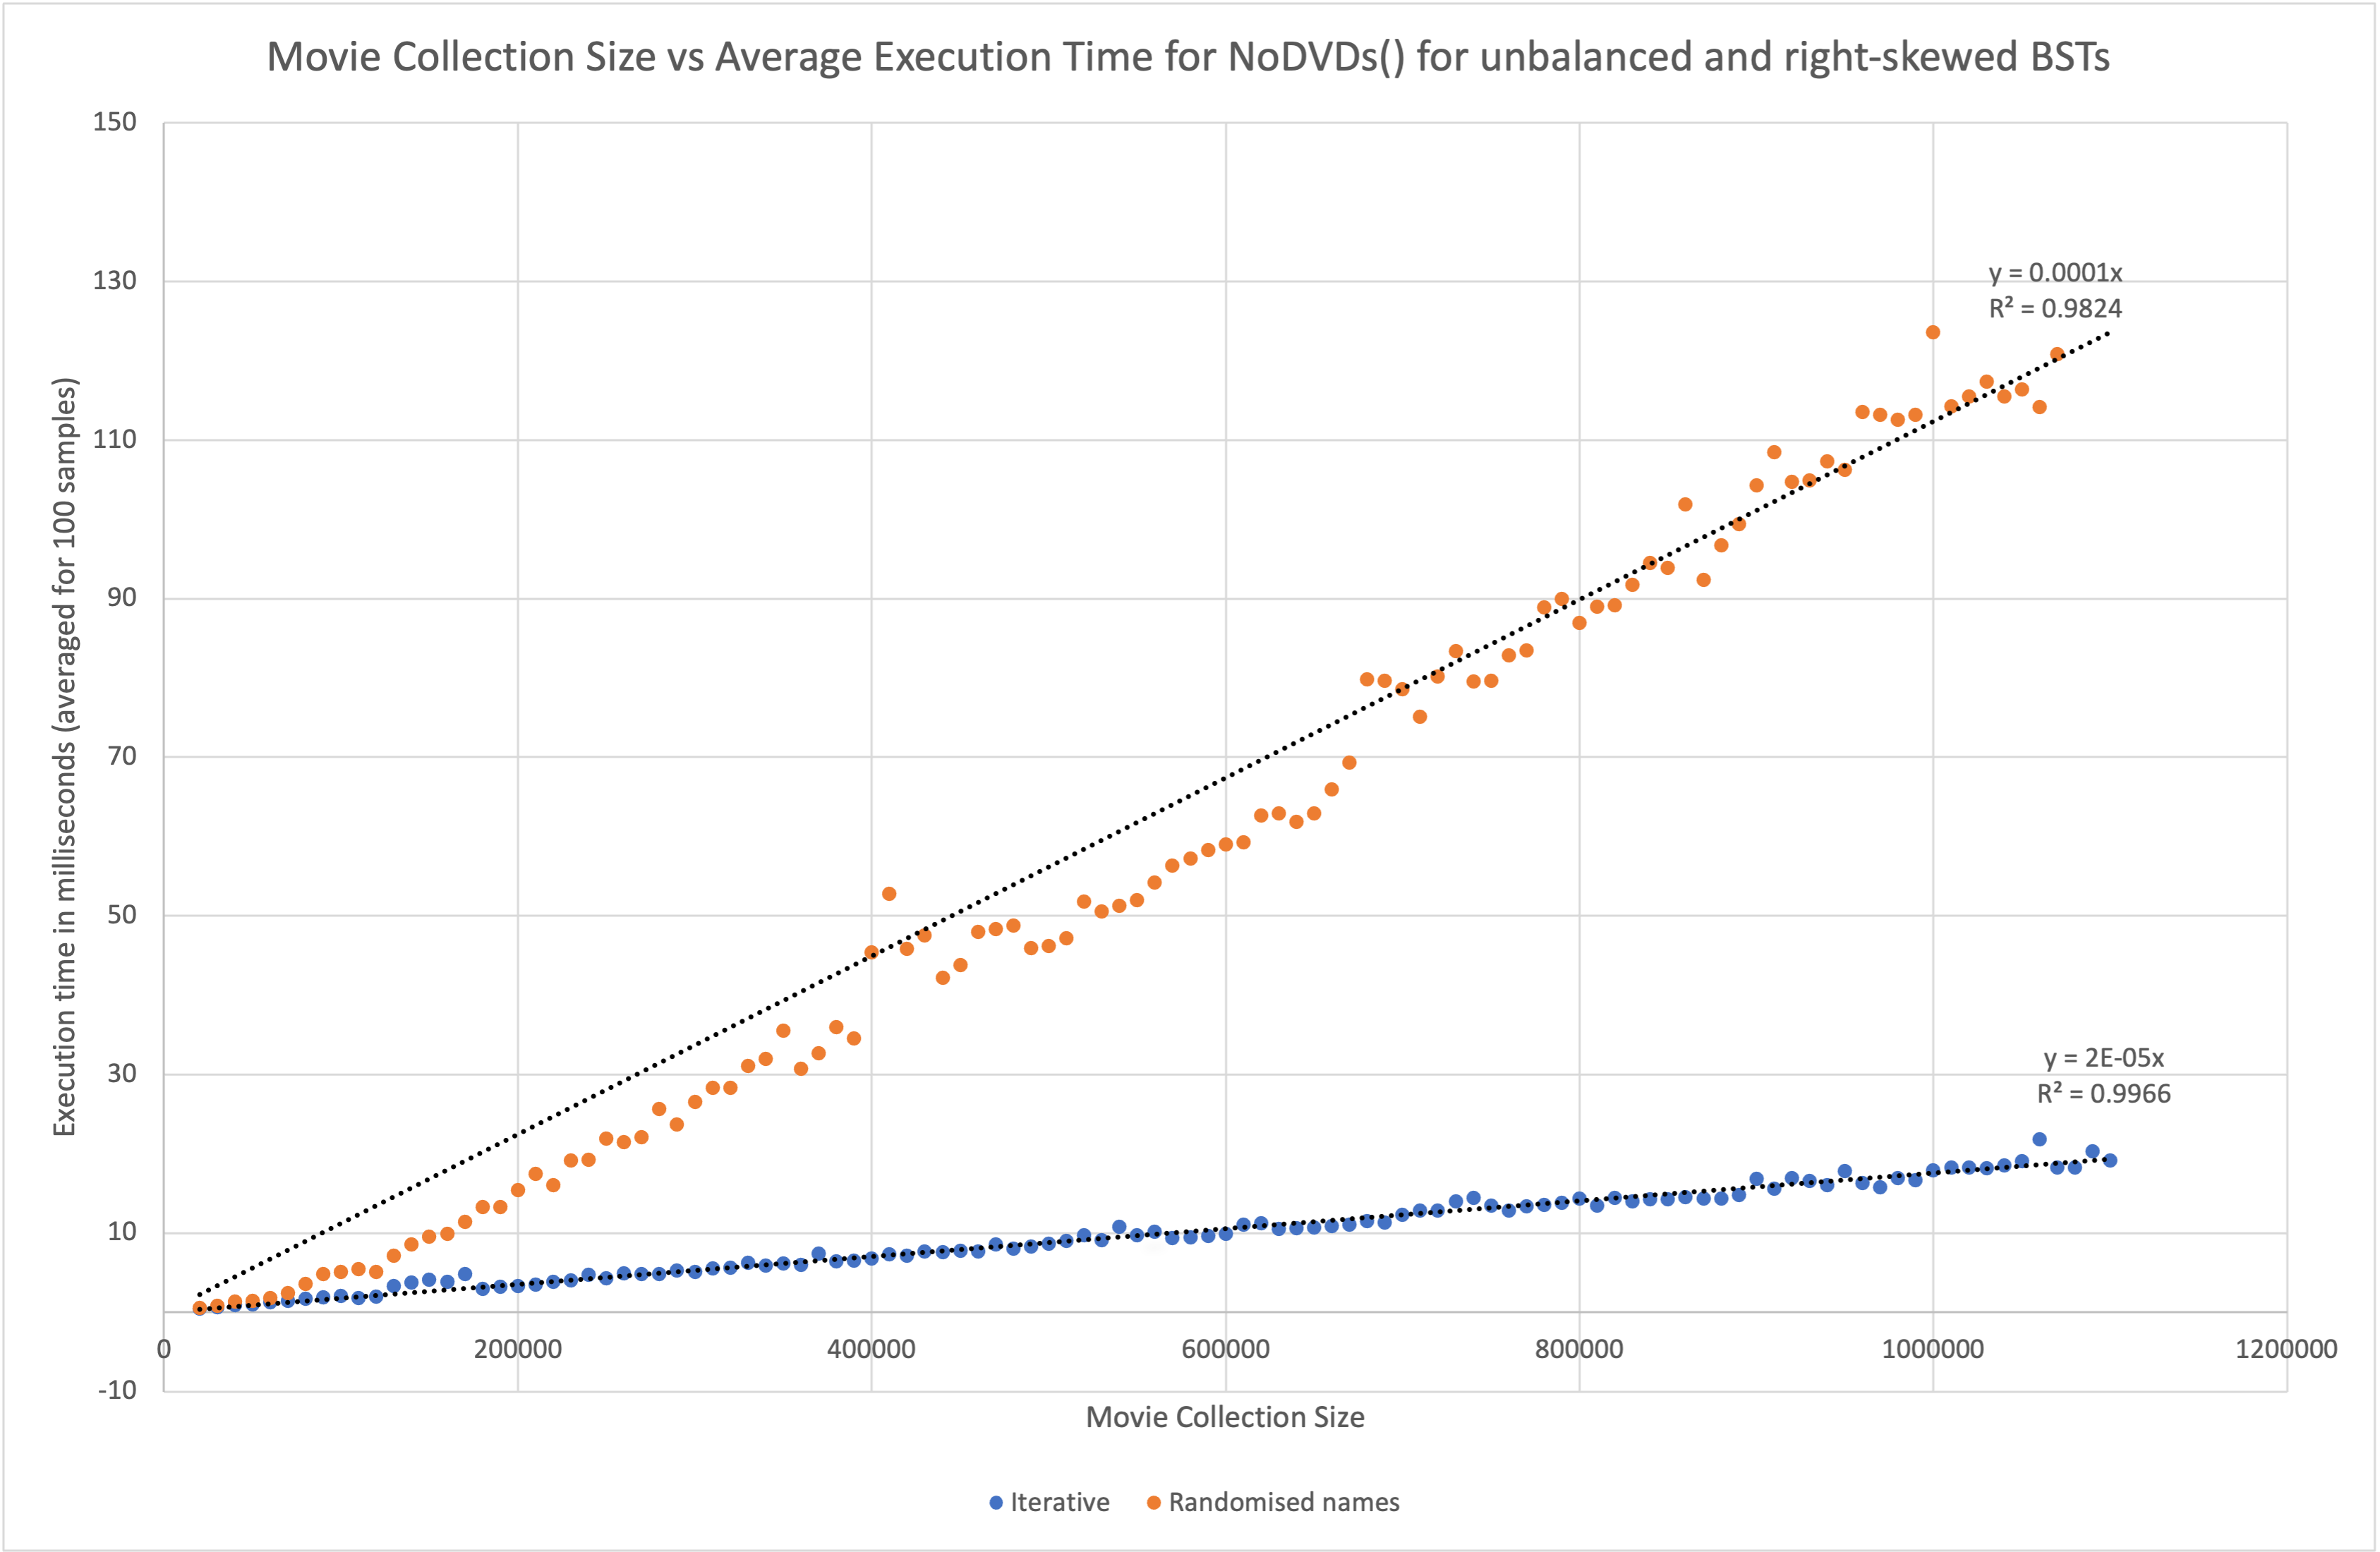
\includegraphics[width=0.7\textwidth]{data/graph_time.png}
\end{wrapfigure}

\noindent
Before looking at ratios between $t(2n)$ and $t(n)$ for the two collection types, it is worth looking at the difference between execution time.

\vspace{3mm}
\noindent
It is clearly evident that the randomised collections take much longer for larger collections. However it seems that for smaller collections; $ \lessapprox 50,000$, the execution time is relatively the same as for iterative collections. It can be extrapolated that this applies to collection sizes smaller than $20,000$ that weren't tested. 
\vspace{3mm}

The iterative collections have a much stronger indication to follow a linear trend with an $R^2$ value of $0.996$ for a linear trend. Random collections seem to somewhat folow a linear trend but the indication is slightly weaker since it has an $R^2$ value of $0.982$. 
\vspace{3mm}

This graph indicates that \codeword{NoDVDs} has a time complexity of $O(n)$ for iterative collections and while the indication is slightly weaker, an $O(n)$ complexity for random names as well. However that the complexity could also be $O(nlogn)$ which is slightly worse than $O(n)$, but not as bad as $O(n^2)$. 
\vspace{3mm}

\noindent
In order to better undestand and hypothesize the likely efficiency classes for the $Iterative$ and $Random$ collections, the ratios between $\frac{t(2n)}{t(n)}$ for each collection size was calculated and graphed.
\vspace{3mm}

\begin{figure}[H]
    \centering
    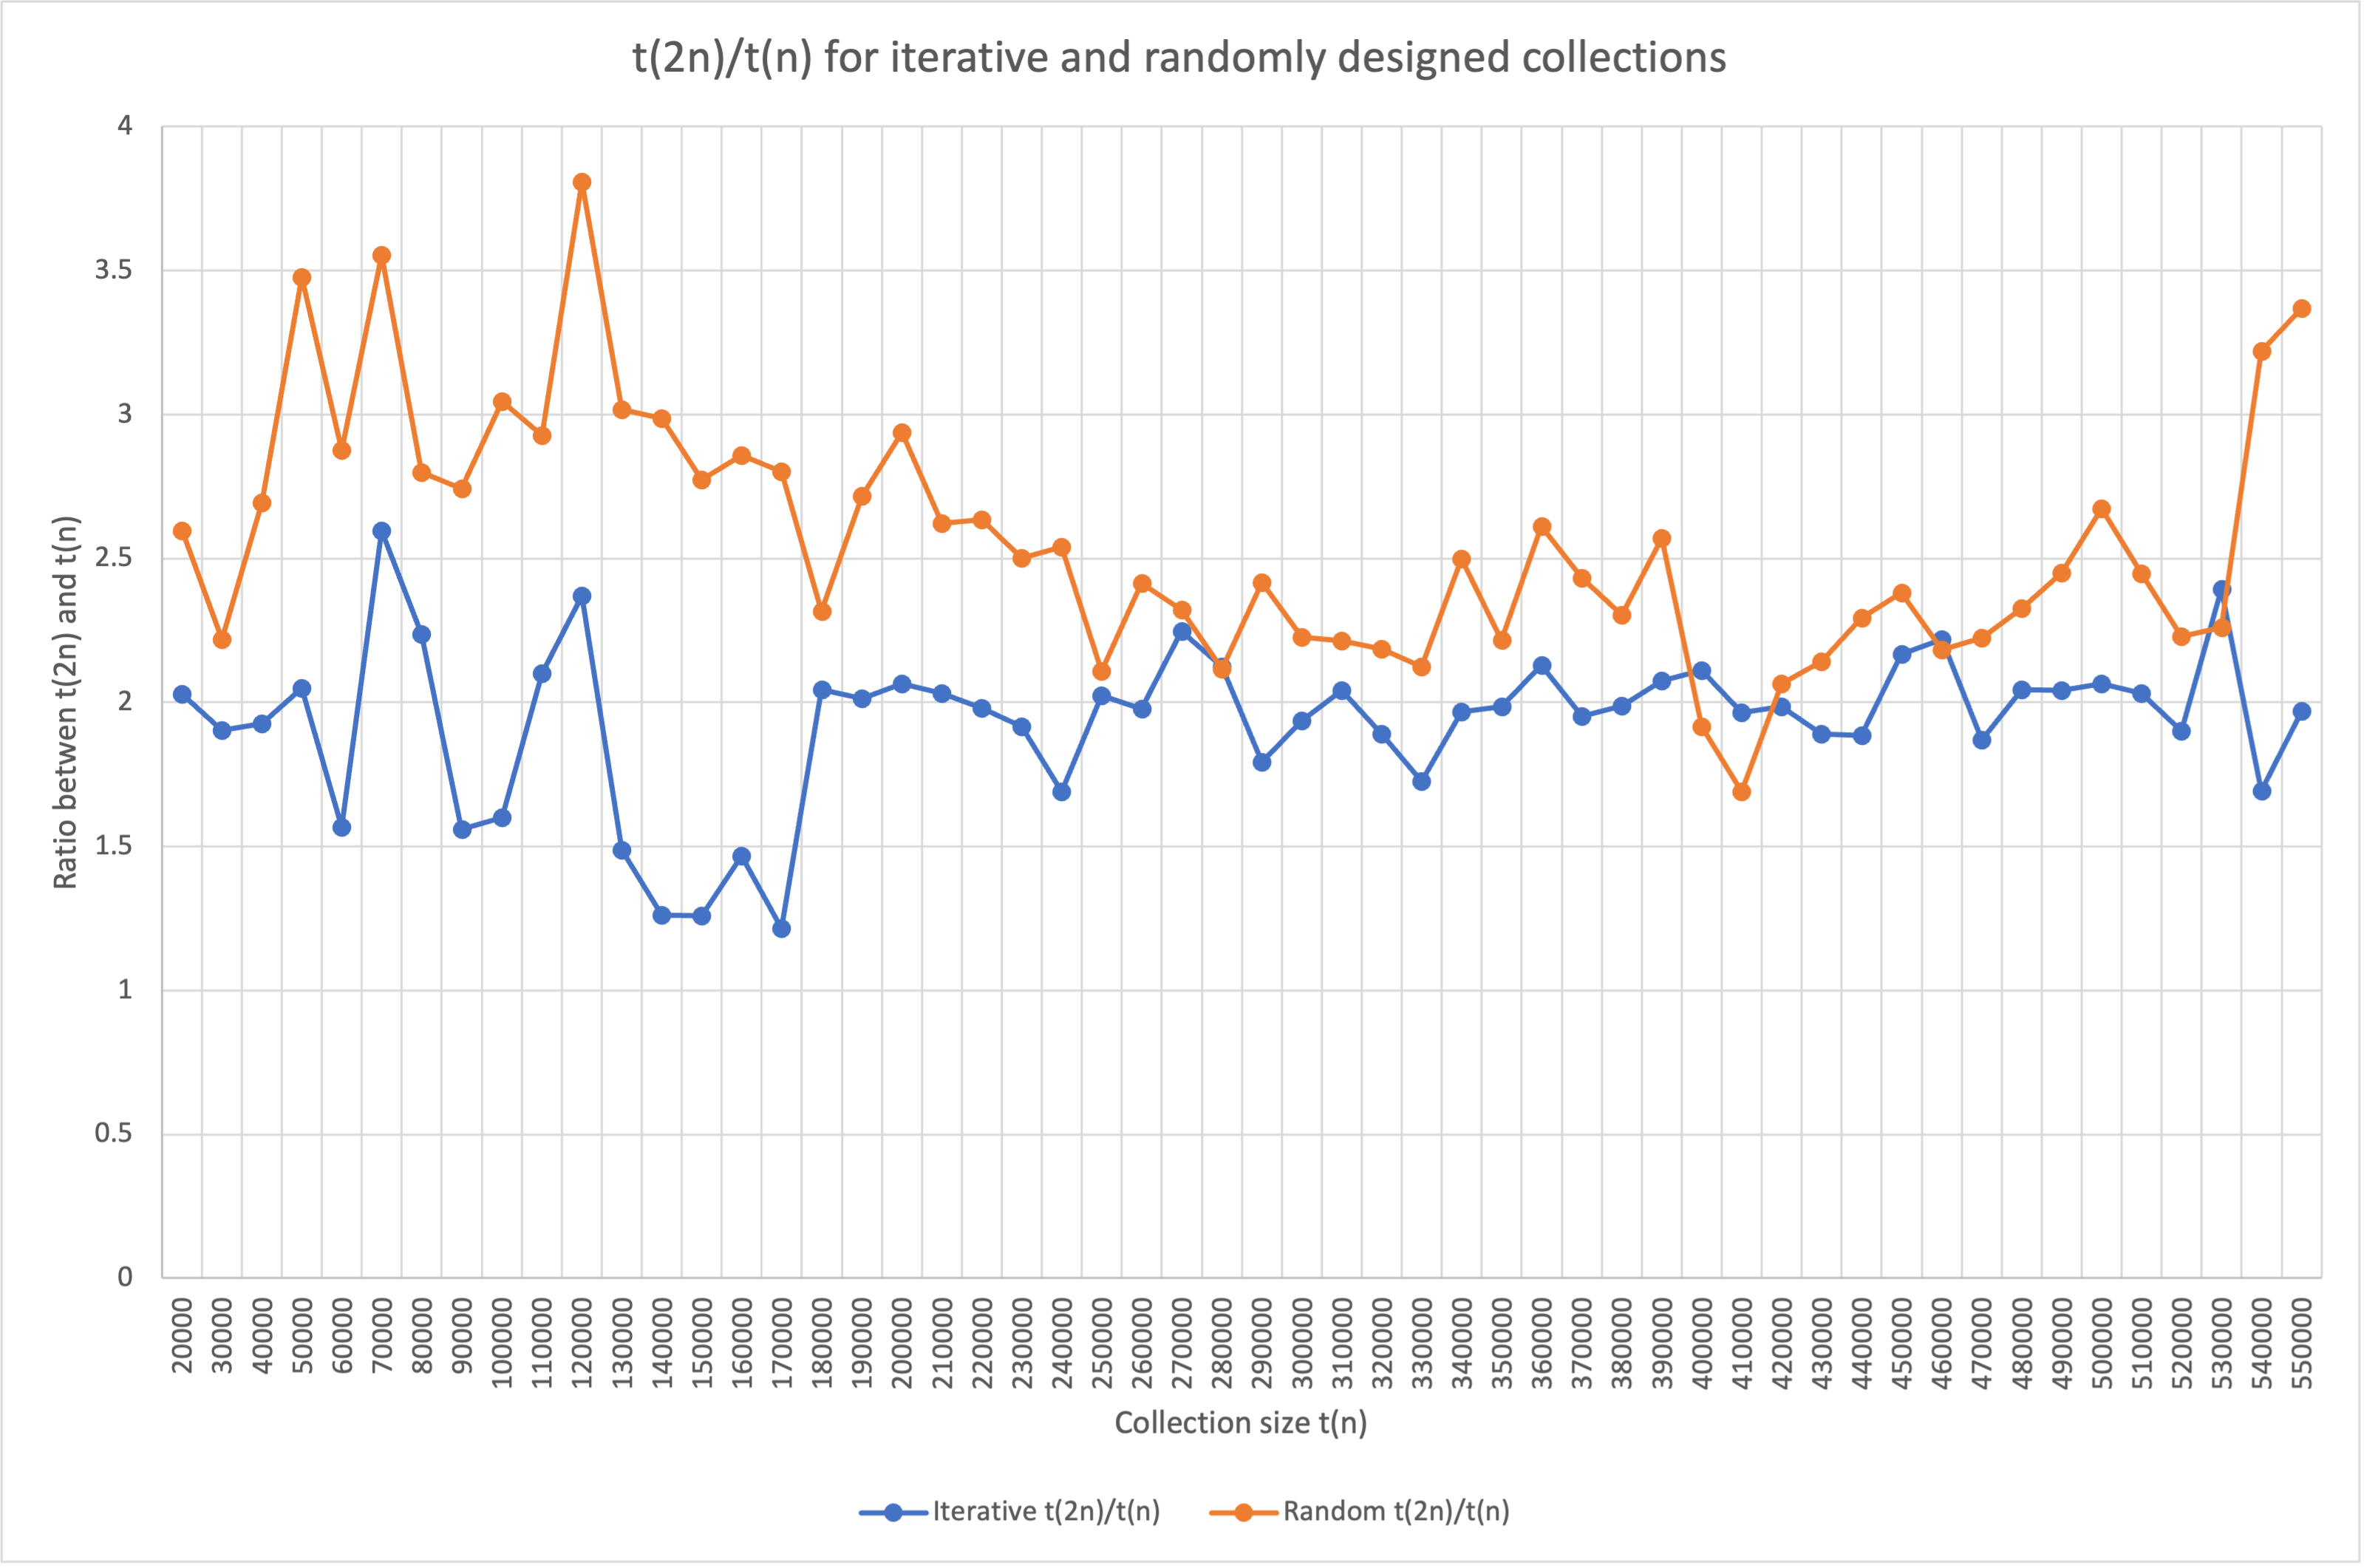
\includegraphics[width=0.8\textwidth]{data/graph_ratios.png}
\end{figure}

\noindent
\textbf{Theoretical Efficiencies}

\noindent
The variance between ratios with the high and low spikes, as  well as the downward trend for the $Random$ ratios may be due to the hardware (and memory) limitations of the computer. It was expected that the ratios would either stay consistent with the theoretical expectations. Theoretically the $Random$ collections will either be unbalanced in the worst case and balanced in the best case. For a balanced cases, the worst efficiency class would be $O(nlogn)$ since each $n$ node would be traversed once and each visit may traverse the height ($logn$) of the tree. The best would  In an unbalanced tree where left or right sub-trees have significant difference in height, or the entire tree is skewed, the worst-case efficiency is $O(n^2)$ since traversing nodes is proportional to the sum of the nodes; $\frac{n(n+1)}{2}$ (Goodrich et al., 2014). 
\vspace{3mm}

\noindent
Thus, it is expected that the efficiency of the $Random$ tests would be $O(n^2)$ or $O(nlogn)$ at their worst and could be $O(n)$ at their best. For the $Iterative$ tests, the best \& worst case would be $O(n)$.
\vspace{3mm}

\noindent
\textbf{Empirical Efficiencies}

\noindent
It can be seen that the iteratively designed (right-skewed) collection has a ratio somewhere between $1.1$ and $2.5$. Ignoring the variance with large collection sizes, it seems that the time efficiency for a right-skewed tree is about $O(n)$ but in some worse seems to be $O(nlogn)$ and some best cases $O(logn)$.
\vspace{3mm}

The randomly designed collection has a higher range between $2$ and about $2.9$. This makes sense since in some of the $100$ tests the tree's could have been relatively balanced, having an efficiency of close to, but above $O(n)$. In some of the worse cases at the left and right sides of the graph, the efficiency is greater than $2.5$ but still less than $4$. This could be due to the tree's being more unbalanced; having greater skews, resulting in the efficiency being much higher than the occurrences when they were closer to $2$. Overall however, it seems that the efficiency class is $O(nlogn)$ when movies have random names. 
\vspace{3mm}

\noindent
\textbf{Summary}

\noindent
Thus based on the empirical analysis, \codeword{NoDVDs} has an efficiency class of $O(nlogn)$. However in the case of randomised names in collections, is bounded by $O(nlogn)$ and $O(n)$, and in the case of right-skewed trees is likely bounded by $O(nlogn)$ and $O(n)$ as well but averages closer to $O(n)$.

\subsubsection{Limitations}
One limitation of this data is that it only provides information on the execution time of the function for a limited number of input sizes. Increasing the range of collection sizes can allow for a much better understanding of the difference between efficiency classes between randomised and right-skewed trees as well as the generalising the efficiency class for \codeword{NoDVDs}.
\vspace{3mm}

\noindent
Additionally tests were conducted on a specific system and environment, and is likely not be representative of the performance on other systems or environments. To overcome this limitation, tests could be conducted on multiple computer systems and IDEs to get a better idea of the range of performance that can be expected.
\vspace{3mm}

\noindent
Furthermore, the specific implementation of the function could also affect its performance. There may be ways to optimize the code or choose a different algorithm that could improve its performance. A non-recursive design using \codeword{Stack} objects could be explored and improvements to code that designs collections could be made.
\vspace{3mm}

\noindent
Additionally, different types of binary search trees such as left-skewed and perfectly balanced trees could be used for the collection design.
\vspace{3mm}

\noindent
Lastly, other techniques for analyzing performance, such as asymptotic analysis, could be used to provide a more theoretical understanding of the function's performance.
\pagebreak

\section{Test Plan}
Testing was done on an M1 Macbook Pro (MacOS Ventura 13.3.1 [22E261]). The test suite was designed using an MSTest project provided by Microsoft in the Visual Studio IDE on the {.}Net 7.0 framework.
\vspace{1.5mm}

\noindent
To ensure that all aspects of the software system cover functional, non-functional and boundary cases of methods, a comprehensive test plan was designed. The plan has been split into three sections that will delve deeper into what was tested each of the three ADTs and why.
\vspace{3mm}

\subsection{Movie ADT}

\subsubsection{CompareTo{(IMovie another)}}
The goal of \codeword{CompareTo} is to return -1 if this movie is less than another by dictionary order, 1 if it is greater, and 0 if it is the same.
\vspace{3mm}

\noindent
Since the movies need to be in dictionary order; the \codeword{String.CompareOrdinal} method was used. In order to test that the method worked properly, an array of movies with titles for each ASCII character from \codeword{space} to \codeword{~} was created. Each movie in the array was in descending order of ASCII value. 
\vspace{3mm}

\noindent
To test if $-1$ was outputted correctly, each \codeword{movie[i]} was \textit{compared to} each movie after it (\codeword{movie[i+1]}) where \codeword{i} ranged from $0$ to the length of the array of movies. It was expected that each comparison would output $-1$ since the movies were already arranged in descending order. This was called \codeword{CompareTo_Lower}.
\vspace{3mm}

\noindent
Similarly, to test if $1$ was outputted correctly, each \codeword{movie[i+1]} was \textit{compared to} each movie before it (\codeword{movie[i]}). Since movies were already arranged in descending order, a movie with a greater array index would have a greater ASCII value. Thus it was expected that each comparison would output $1$. This was called \codeword{CompareTo_Upper}
\vspace{3mm}

\noindent
To test if a movie titled compared to itself is $0$, each movie in the array was compared to itself. To ensure that the method didn't return $0$ because the movie had the same reference, a different array with the the same movies (but different objects) was also used. It was expected that each movie compared to a different movie instance, but with the same titles, would also output $0$. This was called \codeword{CompareTo_Same_with_same_object} and \codeword{CompareTo_Same_with_different_object} respectively. 
\vspace{1mm}

\noindent
From the below summary it can be seen that all tests passed and the method performend as required. These 4 tests can be found in the \hyperlink{subsubsection.5.1.1}{appendix for CompareTo}.
\vspace{3mm}

\noindent
\textbf{Unit testing summarisation}
\begin{figure}[H]
   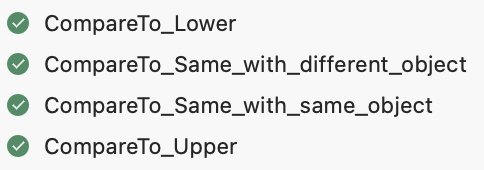
\includegraphics[height=2cm]{/Users/shridhar/Library/CloudStorage/OneDrive-QueenslandUniversityofTechnology/Bachelor of Mathematics and Information Technology/Year 4/CAB301 Algorithms/Assignment 2/Report/data/Summary-CompareTo.png}
\end{figure}

\subsubsection{ToString{()}}
ToString simply needed to output some of the properties of a movie. Hence there were only three tests; testing a movie will all properties defined, with only the movie title defined, and a movie with a null title (as this is the only property that can be set to null). The test data, results and testing code can be found in the \hyperlink{subsubsection.5.1.2}{appendix for ToString}. From the below summary it can be seen that all tests passed and the method performend as required.
\vspace{3mm}

\noindent
\textbf{Unit testing summarisation}
\begin{figure}[H]
   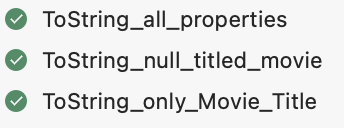
\includegraphics[height=1.8cm]{/Users/shridhar/Library/CloudStorage/OneDrive-QueenslandUniversityofTechnology/Bachelor of Mathematics and Information Technology/Year 4/CAB301 Algorithms/Assignment 2/Report/data/Summary-ToString.png}
\end{figure}

\subsection{MovieCollection ADT}
Since the methods implementated in the \codeword{MovieCollection} ADT all involve Movies and collecitons of Movies, they all used the same data; ofcourse, not all tests used all of the data. As the genre, classification, duration and available copies/total copies aren't relevant to the methods tested, they are kept constant for each different movie object. Additionally, \textit{single collection} refers to a collection with one movie and a \textit{large collection} is a collection with more than one movie.
\vspace{3mm}

\noindent
\textbf{Common Test Data}
\begin{figure}[H]
    \centering
    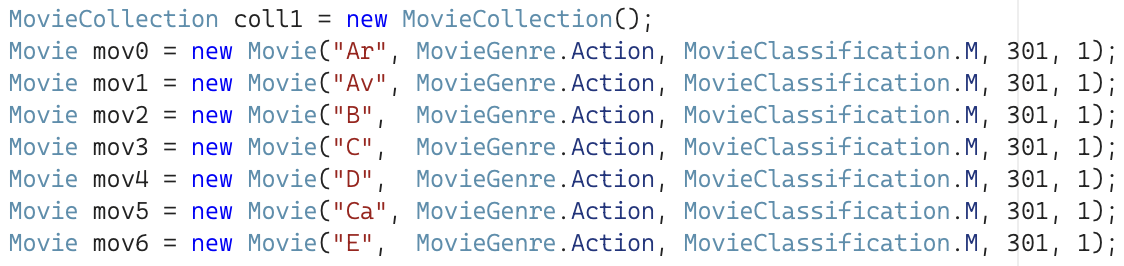
\includegraphics[height=3.2cm]{/Users/shridhar/Library/CloudStorage/OneDrive-QueenslandUniversityofTechnology/Bachelor of Mathematics and Information Technology/Year 4/CAB301 Algorithms/Assignment 2/Report/data/Common-data.png}
\end{figure}

\subsubsection{IsEmpty{()}}
\codeword{IsEmpty} was required to simply return \codeword{true} if a colection had no movies and \codeword{false} otherwise.

\begin{enumerate}
   \item \codeword{IsEmpty_True_empty_collection}: 
   
   \indent{
   Where the method returns \codeword{true} for an empty collection}
   \item \codeword{IsEmpty_True_after_deleting_single_collection}: 
   
   \indent{
   Where the method returns \codeword{true} after deleting the one movie in the collection.}
   \item \codeword{IsEmpty_True_after_deleting_large_collection}: 
   
   \indent{
      Where the method returns \codeword{true} after deleting all the movies in the collection.}
   \item \codeword{IsEmpty_False_single_collection}:
   
   \indent{
   Where the method returns \codeword{false} for a collection with one movie.
   }
   \item \codeword{IsEmpty_False_large_collection}: 
   
   \indent{Where the method returns \codeword{false} for a collection with lots of movie.}
\end{enumerate}
Technically testing the output to be \codeword{false} for a non-empty collection after all of its movie were deleted is not required since it uses another method; \codeword{Clear}. \codeword{Clear} was already tested to work correctly, hence it was used in the \codeword{IsEmpty} testing. Additionally, testing the output to be \codeword{true} when inserting multiple movies was also unnecessary since the number of movies will be greater than zero whether one or a million movies exist in a collection. However due to their trivial nature (and to prevent losing marks), they were still included. 

Additionally, for each of these tests, the post-condition that the the \codeword{count} property (read outside of the \textit{MovieCollection} class using the \codeword{Number} field) doesn't change before and after \codeword{IsEmpty} is called, was also checked.
\vspace{4mm}

\noindent
From the below summary it can be seen that all tests passed and the method performend as required. The test data, results and testing code can be found in the \hyperlink{subsubsection.5.2.1}{appendix for IsEmpty}. 
\vspace{1mm}

\noindent
\textbf{Unit testing summarisation}
\begin{figure}[H]
   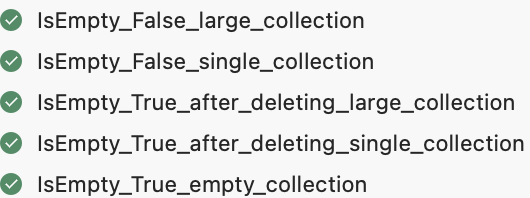
\includegraphics[height=2.3cm]{/Users/shridhar/Library/CloudStorage/OneDrive-QueenslandUniversityofTechnology/Bachelor of Mathematics and Information Technology/Year 4/CAB301 Algorithms/Assignment 2/Report/data/Summary-IsEmpty.png}
\end{figure}

\subsubsection{Insert{(IMovie movie)}}
The first test involved inserting a \codeword{root} to an empty collection and was done to ensure that the method correctly sets the \codeword{root} variable to the new movie. This is important as in this assignment a tree can only be traversed if the root is defined. This test was expected to return \codeword{true};
\vspace{2mm}

\noindent
The next two tests involed testing whether a \codeword{LChild} and \codeword{RChild} were inserted correctly and that the method returns \codeword{true}. Where a \codeword{RChild} must be greater than the root and the \codeword{LChild} is less than it in dictionary order. This is important to determine whether the collection is created correctly. It is worth mentioning, this test was done by checking whether the \codeword{Insert} method writes \codeword{`movie is a RChild'} or \codeword{`movie is a LChild'} into a line in the Visual Studio `console' for a given \codeword{movie} parameter that is inserted successfully.
\vspace{2mm}

\noindent
Next, it was tested whether trying to insert a movie that already exists in a single collection returns \codeword{false} and the movie is not inserted (by checking if \codeword{Number} is invariant).
\vspace{2mm}

\noindent
Lastly, as a sanity check, it was tested whether inserting multiple movies all outputted true. It is worth noting that testing insertion of multiple movies is not required. This is because inserting a movie into a Binary Search Tree is never done between existing movie but only as leaves. For example, if collection has a \codeword{root} as `Batman' and it's \codeword{RChild} was `Dungeons and Dragons'. Then inserting `Cars' wouldn't make it the new \codeword{RChild} of `Batman' but the \codeword{LChild} of `Dungeons and Dragons'. 
\vspace{2mm}

\noindent
Additionally, for each of test, the post-condition was tested --- that the \codeword{Number} of movies of increments by 1 if \codeword{Insert} is successful (returns \codeword{true}) and doesn't change if it is unsuccessfull (returns \codeword{false}).
\vspace{2mm}

\noindent
From the below summary it can be seen that all tests passed and the method performend as required.
\vspace{4mm}

\noindent
These tests were names intuitively are summarised below. Test data, results and testing code can be found in the \hyperlink{subsubsection.5.2.2}{appendix for Insert}.
\vspace{1mm}

\noindent
\textbf{Unit testing summarisation}
\begin{figure}[H]
   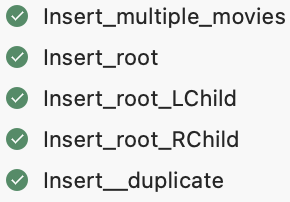
\includegraphics[height=2.8cm]{/Users/shridhar/Library/CloudStorage/OneDrive-QueenslandUniversityofTechnology/Bachelor of Mathematics and Information Technology/Year 4/CAB301 Algorithms/Assignment 2/Report/data/Summary-Insert.png}
\end{figure}

\subsubsection{ToArray{()}}
The \codeword{ToArray} method simply returns an \codeword{IMovie} array containing \codeword{Movie} objects, sorted in dictionary order. Thus, testing involved checking if the sorting was correct for a \textit{single} collection and \textit{large} collection, as well as for an empty collection; in which case the output was expected to be an empty \codeword{IMovie} array (i.e. \codeword{new IMovie[0]}). 
\vspace{1mm}

\noindent
The below summary shows these three all passed. Test data, results and code can be found in the \hyperlink{subsubsection.5.2.3}{appendix for ToArray}.
\vspace{2mm}

\noindent
\textbf{Unit testing summarisation}
\begin{figure}[H]
   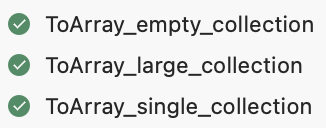
\includegraphics[height=1.8cm]{/Users/shridhar/Library/CloudStorage/OneDrive-QueenslandUniversityofTechnology/Bachelor of Mathematics and Information Technology/Year 4/CAB301 Algorithms/Assignment 2/Report/data/Summary-ToArray.png}
\end{figure}
\pagebreak

\subsubsection{Search{(string title)}}
The \codeword{Search} method was designed to return a reference to an \codeword{IMovie} object if the movie is in `\codeword{this}' movie collection and \codeword{null} otherwise. A number of tests were designed to ensure these conditions were met.
\vspace{3mm}

\noindent
To test if the correct ouput was \codeword{null}, the method was tested against an empty collection with a \codeword{non-null} \textbf{title}, a \textit{single} and \textit{large} collection with a \codeword{null} \textbf{title} as well as a \textbf{title}; that is not in either collection. 
\vspace{3mm}

\noindent
To test if the correct output was a reference, the method was tested using a movie \textbf{title} known to exist in a \textit{single} and a \textit{large} collection.
\vspace{1mm}

\noindent
Of course, the post-condition that the \codeword{Number} of movies remains unchanged and the object passed is a reference rather tha independent copy, was also checked for each of the 7 tests. As summarised below, each of these tests passed. Test data, results and code can be found in the \hyperlink{subsubsection.5.2.4}{appendix for Search}.
\vspace{2mm}

\noindent
\textbf{Unit testing summarisation}
\begin{figure}[H]
   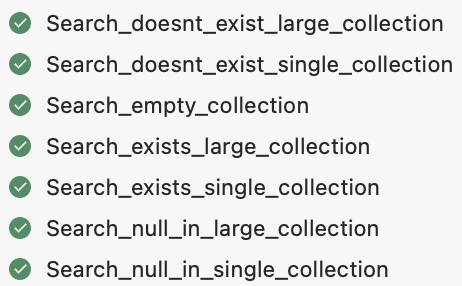
\includegraphics[height=3.5cm]{/Users/shridhar/Library/CloudStorage/OneDrive-QueenslandUniversityofTechnology/Bachelor of Mathematics and Information Technology/Year 4/CAB301 Algorithms/Assignment 2/Report/data/Summary-Search.png}
\end{figure}

\subsubsection{Delete{(IMovie movie)}}
If the parameter \codeword{movie} is in the collection, the \codeword{Delete} method would remove it and return \codeword{true} and decrement the \codeword{Number} value by 1 and return \codeword{false} otherwise while also leaving the \codeword{Number} parameter unchanged.
\vspace{1mm}

Additionally, it was assumed that when deleting a node (movie) that isn't a leaf and has two children, it would be replaced by the \textit{right most node in the left sub-tree} of that node; similar to lecture material. It is worth mentioning that \codeword{ToArray} was used to test if the structure of the collection was preserved.
\vspace{2mm}


\noindent
For the tests where the method returned \codeword{false} the post-condition that the \codeword{Number} of movies is unchanged ($oldNumber = newNumber$) and that the collection remains unchanged (\codeword{ToArray} is the same before and after false deletion) was checked.
\vspace{1.5mm}

For the tests where \codeword{Delete} was \codeword{true}, the post-condition that the deleted movie could no longer be found in the collection (using \codeword{Search}); signifying that it was correctly set to null and no longer exists was checked. The other post-condition that \codeword{Number} decrements (i.e $oldNumber=newNumber+1$) was checked.

\noindent
The 13 tests can be summarised below. Note that for \textbf{9} to \textbf{13}, the deleted \codeword{node} is not a leaf or a root for the collection. 
\begin{enumerate}
   \item \codeword{Delete_node_not_in_single_collection}
   
   \indent{Where the method returns \codeword{false} when the movie is not in a collection with one movie.}
   \item \codeword{Delete_node_not_in_large_collection}
   
   \indent{Where the method returns \codeword{false} when the movie is not in a collection with multiple movies}
   \item \codeword{Delete_node_not_in_empty_collection.}
   
   \indent{Where the method returns \codeword{false} when the movie is not in an empty collection.}
   \item \codeword{Delete_null_node_in_single_collection}
   
   \indent{Where the method returns \codeword{false} when the movie is \codeword{null} for a collection with only one movie.}
   \item \codeword{Delete_root_single_collection}
   
   \indent{Where the method returns \codeword{true} when the movie is deleted from a collection with only one movie.}
   \item \codeword{Delete_root_has_only_LChild}
   
   \indent{Where the method returns \codeword{true} when the movie is deleted from a collection with only a \codeword{root} and its \codeword{LChild}. The new root is the deleted node's \codeword{LChild}; confirmed by checking if \codeword{Search}-ing for \codeword{LChild} is \codeword{true} since \codeword{Search} traverses the collection starting at the \codeword{root}.}
   \item \codeword{Delete_root_has_only_RChild}
   
   \indent{Where the method returns \codeword{true} when the movie is deleted from a collection with only a \codeword{root} and its \codeword{RChild}. The new root is the deleted node's \codeword{RChild}; confirmed by checking if \codeword{Search}-ing for \codeword{LChild} is \codeword{true} since \codeword{Search} traverses the collection starting at the \codeword{root}.}
   \item \codeword{Delete_root_has_LChild_and_RChild_as_leaves}
   
   \noindent{Where the method returns \codeword{true} when the \codeword{root} is deleted from a collection with a \codeword{root} having  \textbf{both} a \codeword{LChild} \textbf{and} \codeword{RChild}. The new root becomes the deleted node's \codeword{LChild}; confirmed by checking if \codeword{coll1.ToArray} is confirmed to be in dictionary order. Since \codeword{ToArray} uses an $In-Order~traversal~method$, if the node was replaced by its \codeword{RChild} the order would then be \textit{D, B} rather than \textit{B, D} which would result from \codeword{LChild} becoming the root}.
   \item \codeword{Delete_node_has_only_LChild_leaf}
   
   \noindent{Where the method returns \codeword{true} when a node that only has a \codeword{LChild} leaf, is deleted. \codeword{LChild} is confirmed to replace it by checking if the \codeword{coll1.ToArray} method doesn't contains a \codeword{null} value, since if the non-existent \codeword{RChild} replaces the node, the collection will have a movie with a \codeword{null} title.}
   \item \codeword{Delete_node_has_only_RChild_leaf}
   
   \noindent{Where the method returns \codeword{true} when a node that only has a \codeword{RChild} leaf, is deleted. \codeword{RChild} is confirmed to replace it by checking if the \codeword{coll1.ToArray} method doesn't contains a \codeword{null} value, since if the non-existent \codeword{LChild} replaces the node, the collection will have a movie with a \codeword{null} title. }
   \item \codeword{Delete_node_has_LChild_and_RChild_as_leaves}
   
   \noindent{Where the method returns \codeword{true} when a node that has a \codeword{RChild} leaf and \codeword{LChild} leaf, is deleted. \codeword{LChild} is confirmed to replace it by checking if the \codeword{coll1.ToArray} method is in dictionary order. Since \codeword{ToArray} uses a $In-Order~traversal~method$, if the node was replaced by its \codeword{RChild} the order would then be \textit{Av, D, B} which is incorrect. And if it was replaced by \codeword{LChild} the order would be \textit{Av, B, D}, which is correct.}
   \item \codeword{Delete_node_has_LChild_with_LeftSkewedtree_and_RChild_as_leaf}
   
   \noindent{Where the method returns \codeword{true} when a node that has a \codeword{RChild} leaf and and a \codeword{LChild} with a left-skewed sub-tree, is deleted, and replaced by the immediate \codeword{LChild}. The replacement is checked to be correct by confirming that \codeword{coll1.ToArray} is in dictionary order. Since \codeword{ToArray} uses an $In-Order~traversal~method$, if the node was replaced by its non-immediate \codeword{LChild}; \codeword{Av}, the order would then be \textit{Ar, B, Av, Ca}--- which is incorrect, rather than \textit{Ar, Av, B, Ca} which would result from the immediate \codeword{LChild} being the replacement.}
   \item \codeword{Delete_node_has_LChild_with_RightSkewedtree_and_RChild_as_leaf}
   
   \noindent{Where the method returns \codeword{true} when a node that has a \codeword{RChild} leaf and and a \codeword{LChild} with a right-skewed sub-tree, is deleted, and replaced by the \textit{right most node in its left sub-tree}. The replacement is checked to be correct by confirming that \codeword{coll1.ToArray} is in dictionary order. Since \codeword{ToArray} uses an $In-Order~traversal~method$, if the node was replaced by its immediate \codeword{LChild}; \codeword{Ar}, the order would then be \textit{B, Av, Ar, D, E}--- which is incorrect, rather than \textit{Av, Ar, B, D, E} which would result from the \textit{right most node in its left sub-tree}; \codeword{B}, being the replacement.}
\end{enumerate}
\noindent
\pagebreak

\noindent
As summarised below, each of these tests passed and the method was confirmed to perform as required. Test data, results and code can be found in the \hyperlink{subsubsection.5.2.5}{appendix for Delete}.
\vspace{2mm}

\noindent
\textbf{Unit testing summarisation}
\begin{figure}[H]
   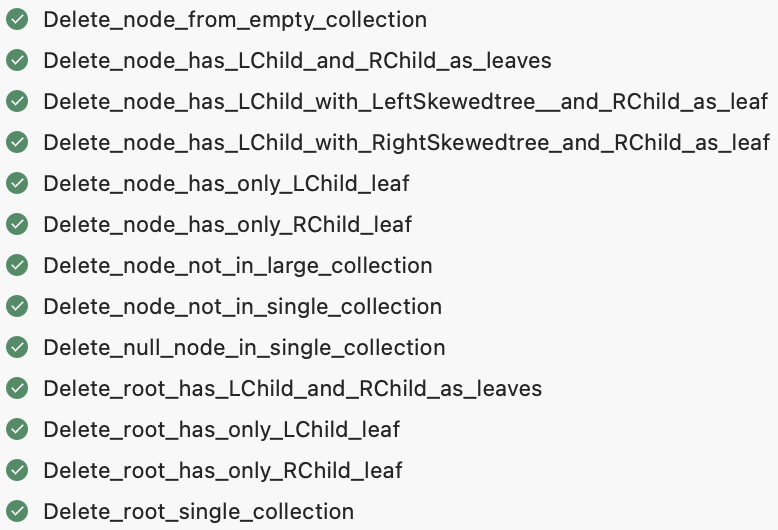
\includegraphics[height=6cm]{/Users/shridhar/Library/CloudStorage/OneDrive-QueenslandUniversityofTechnology/Bachelor of Mathematics and Information Technology/Year 4/CAB301 Algorithms/Assignment 2/Report/data/Summary-Delete.png}
\end{figure}

\subsubsection{Clear{()}}
The \codeword{Clear} method simply sets the root of a BST as null and the garbage collector for C\# in Visual Studio erases all other nodes from memory. Thus three tests were only needed. Testing involved clearing an empty array, clearing a \textit{single} collection and clearing a \textit{large} collection while checking if the \codeword{Number} property becomes 0 for each of them. 
\vspace{1mm}

\noindent
From the below summary it can be seen that all tests passed and the method performend as required. Test data, results and testing code can be found in the \hyperlink{subsubsection.5.2.6}{appendix for Clear}.
\vspace{2mm}

\noindent
\textbf{Unit testing summarisation}
\begin{figure}[H]
   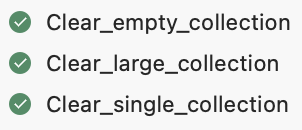
\includegraphics[height=1.8cm]{/Users/shridhar/Library/CloudStorage/OneDrive-QueenslandUniversityofTechnology/Bachelor of Mathematics and Information Technology/Year 4/CAB301 Algorithms/Assignment 2/Report/data/Summary-Clear.png}
\end{figure}

\subsubsection{NoDVDs}
This method simply outputted the sum of \codeword{TotalCopies} for each movie in the collection. Since \codeword{Insert} and \codeword{Delete} were already tested to perform as specified, there was no need to test \codeword{NoDVDs} before and after inserting or deleting. Hence it was simply tested for 3 static collections; an empty, \textit{single} and \textit{large} collection.
\vspace{1mm}

\noindent
From the below summary it can be seen that all tests passed and the method performend as required. Test data, results and testing code can be found in the \hyperlink{subsubsection.5.2.7}{appendix for Clear}.
\vspace{2mm}

\noindent
\textbf{Unit testing summarisation}
\begin{figure}[H]
   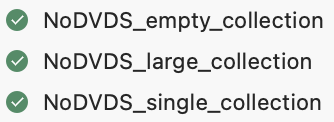
\includegraphics[height=1.6cm]{/Users/shridhar/Library/CloudStorage/OneDrive-QueenslandUniversityofTechnology/Bachelor of Mathematics and Information Technology/Year 4/CAB301 Algorithms/Assignment 2/Report/data/Summary-NoDVDs.png}
\end{figure}


\section{References}

Goodrich, M. T., Tamassia, R., \& Goldwasser, M. H. (2014). Data structures and algorithms in Java (6th ed.). John Wiley \& Sons.http://bedford-computing.co.uk/learning/wp-content/uploads/2016/08/Data-Structures-and-Algorithms-in-Java-6th-Edition.pdf
\pagebreak

\section{Appendix}

\subsection{Movie ADT}
\subsubsection{CompareTo{(IMovie another)}}
\hyperlink{subsubsection.3.1.1}{Back to test plan for CompareTo}.
\begin{figure}[H]
    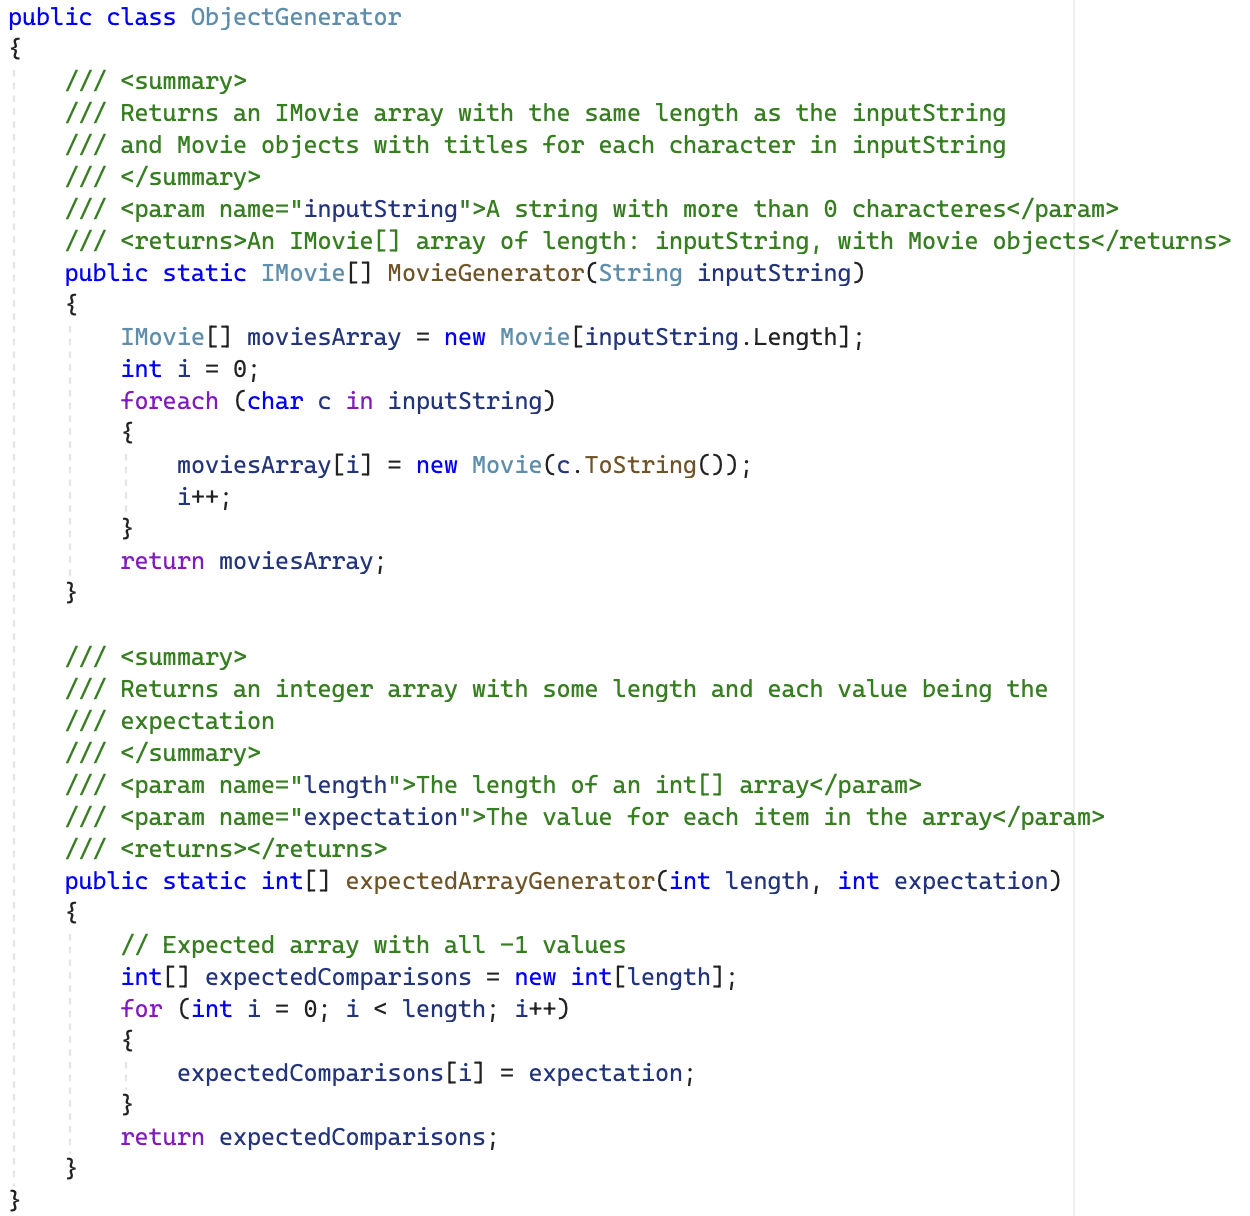
\includegraphics[height=11cm]{data/ObjectGenerator.png}
    \caption{Helper class for CompareTo testing}
\end{figure}
\begin{figure}[H]
    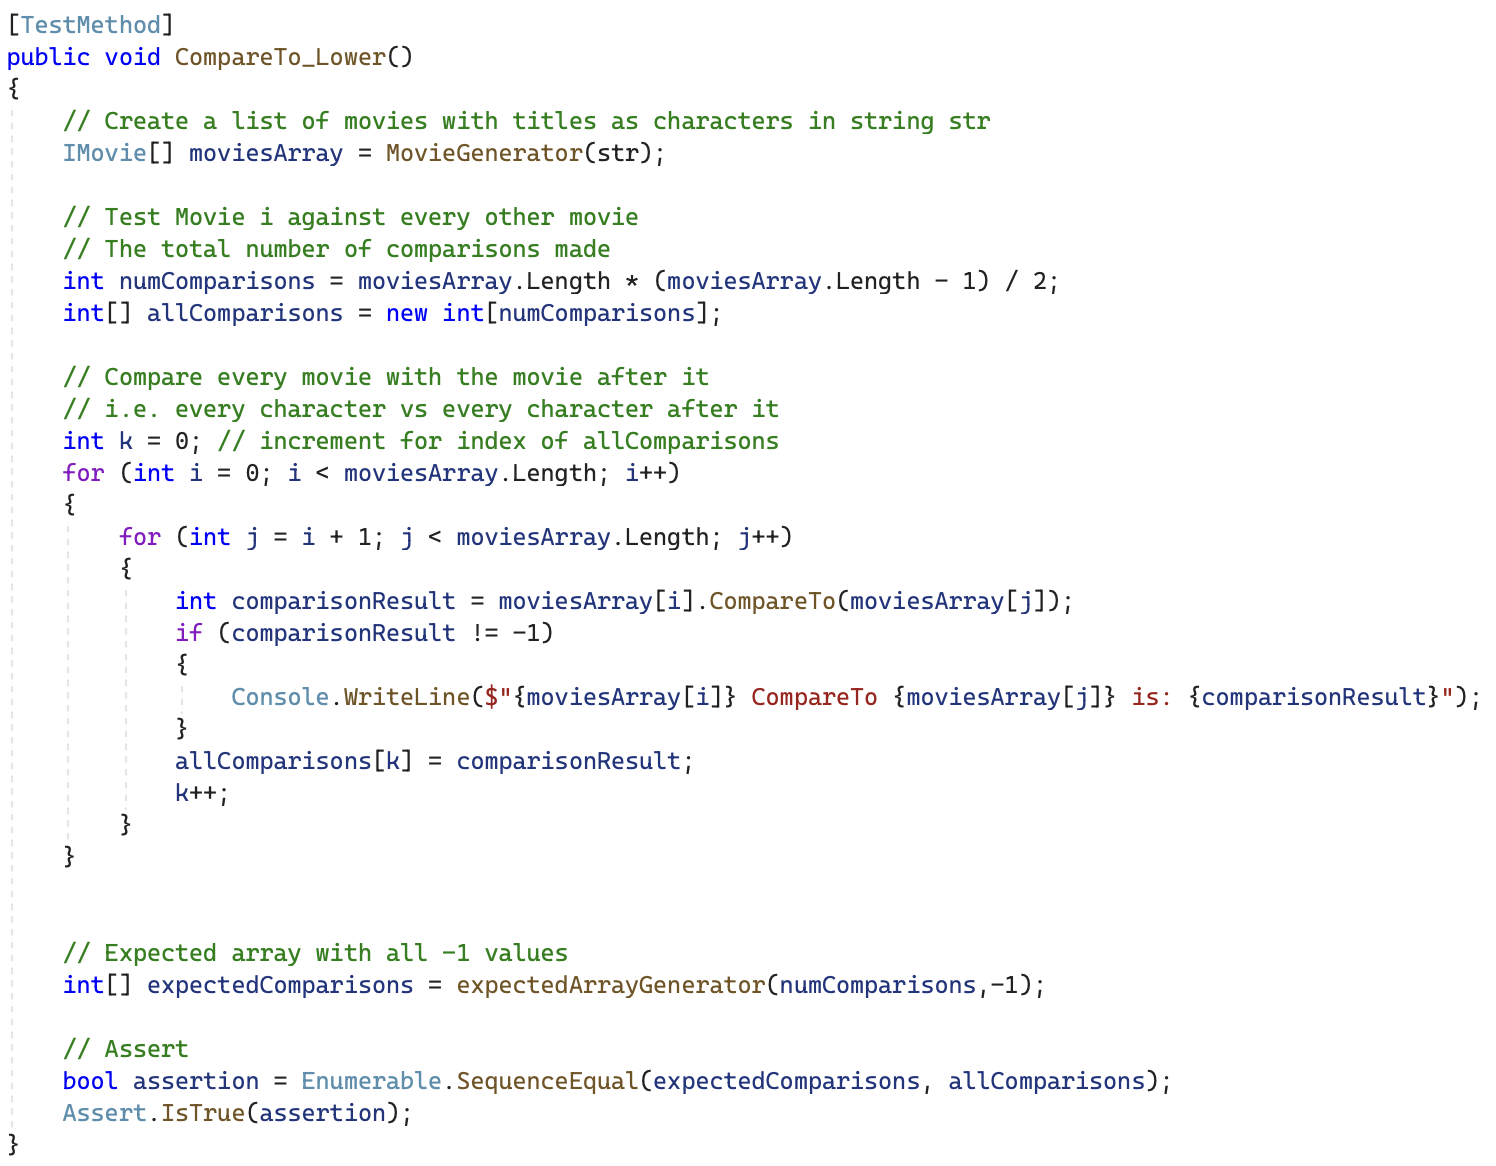
\includegraphics[height=12cm]{data/CompareTo_Lower.png}
    \caption{Test for testing if $-1$ is outputted correctly for all possible comparisons}
\end{figure}
\begin{figure}[H]
    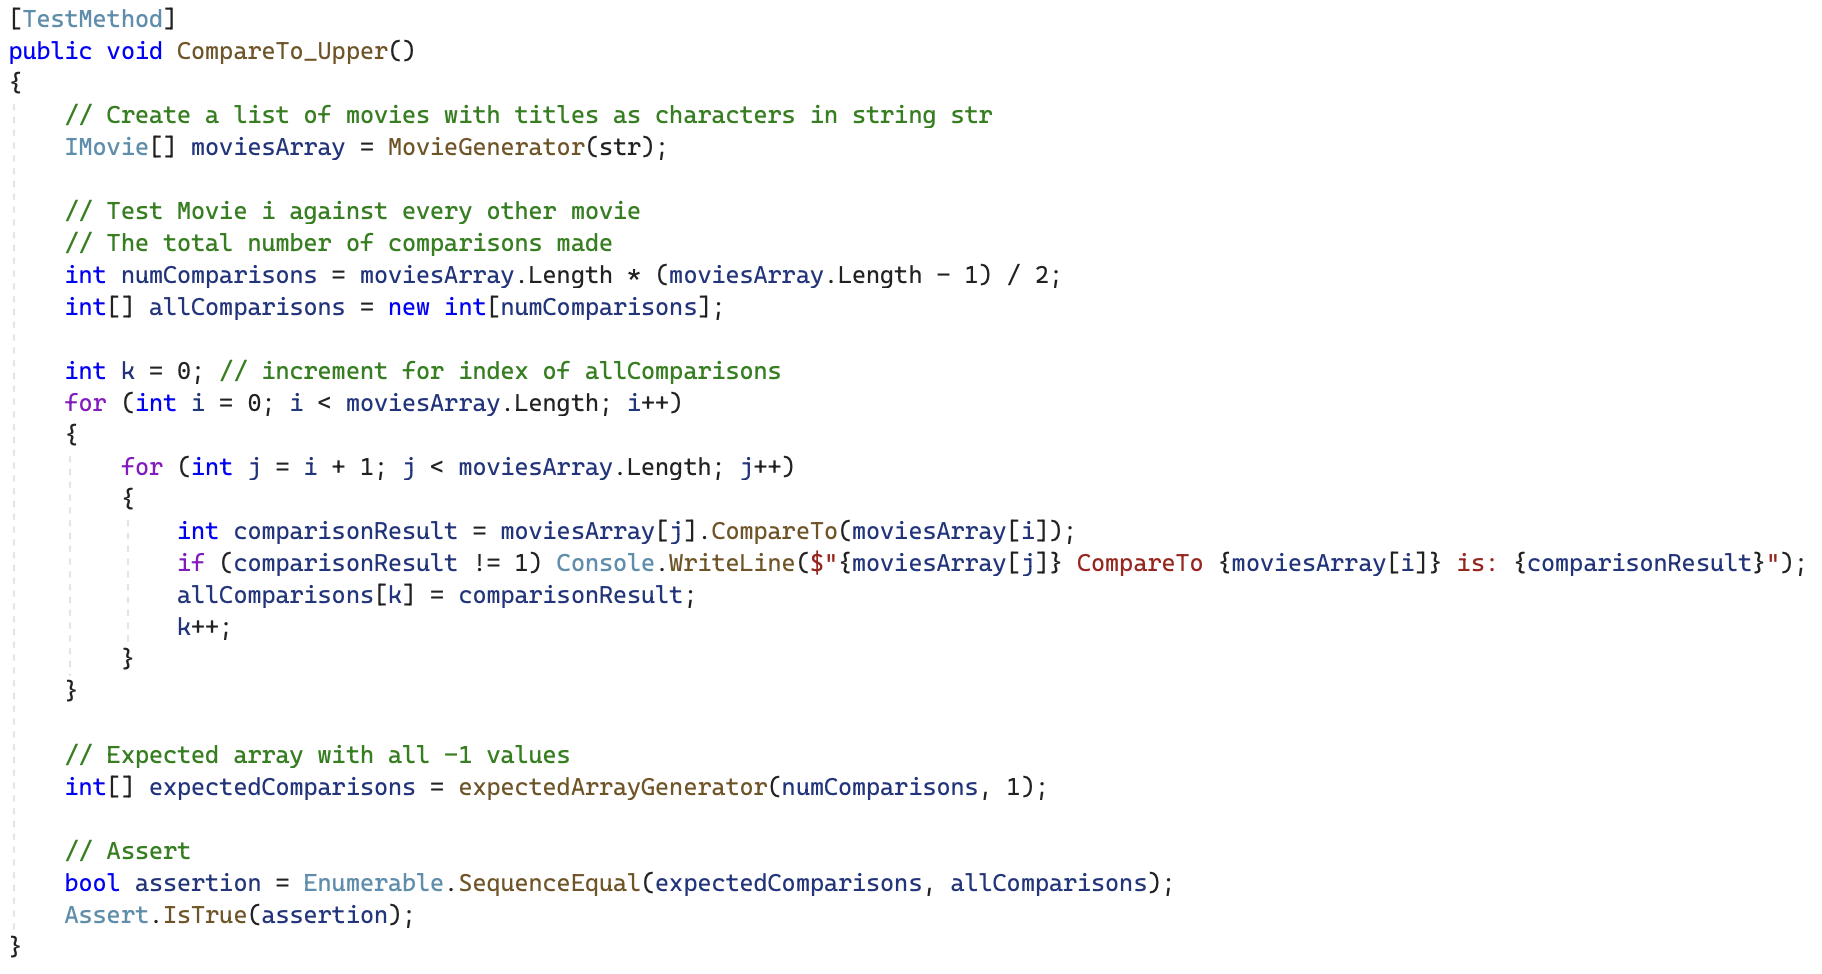
\includegraphics[height=10cm]{data/CompareTo_Upper.png}
    \caption{Test for testing if $1$ is outputted correctly for all possible comparisons}
\end{figure}
\begin{figure}[H]
    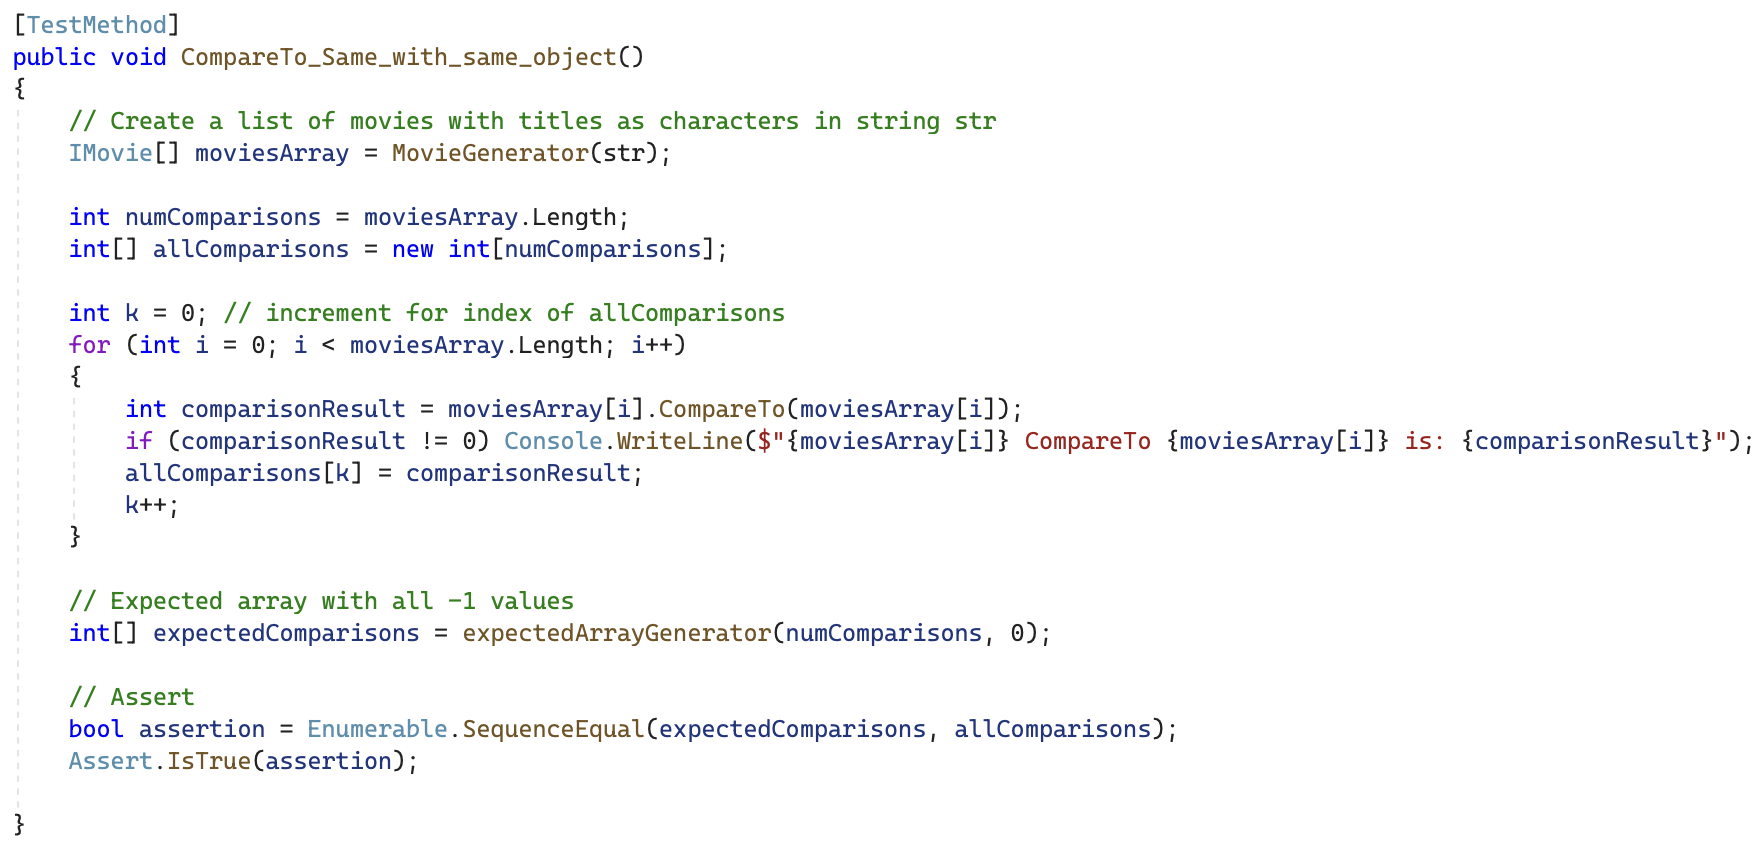
\includegraphics[height=8cm]{data/CompareTo_Same_with_same_object.png}
    \caption{Test for testing if $0$ is outputted correctly for all possible comparisons}
\end{figure}
\begin{figure}[H]
    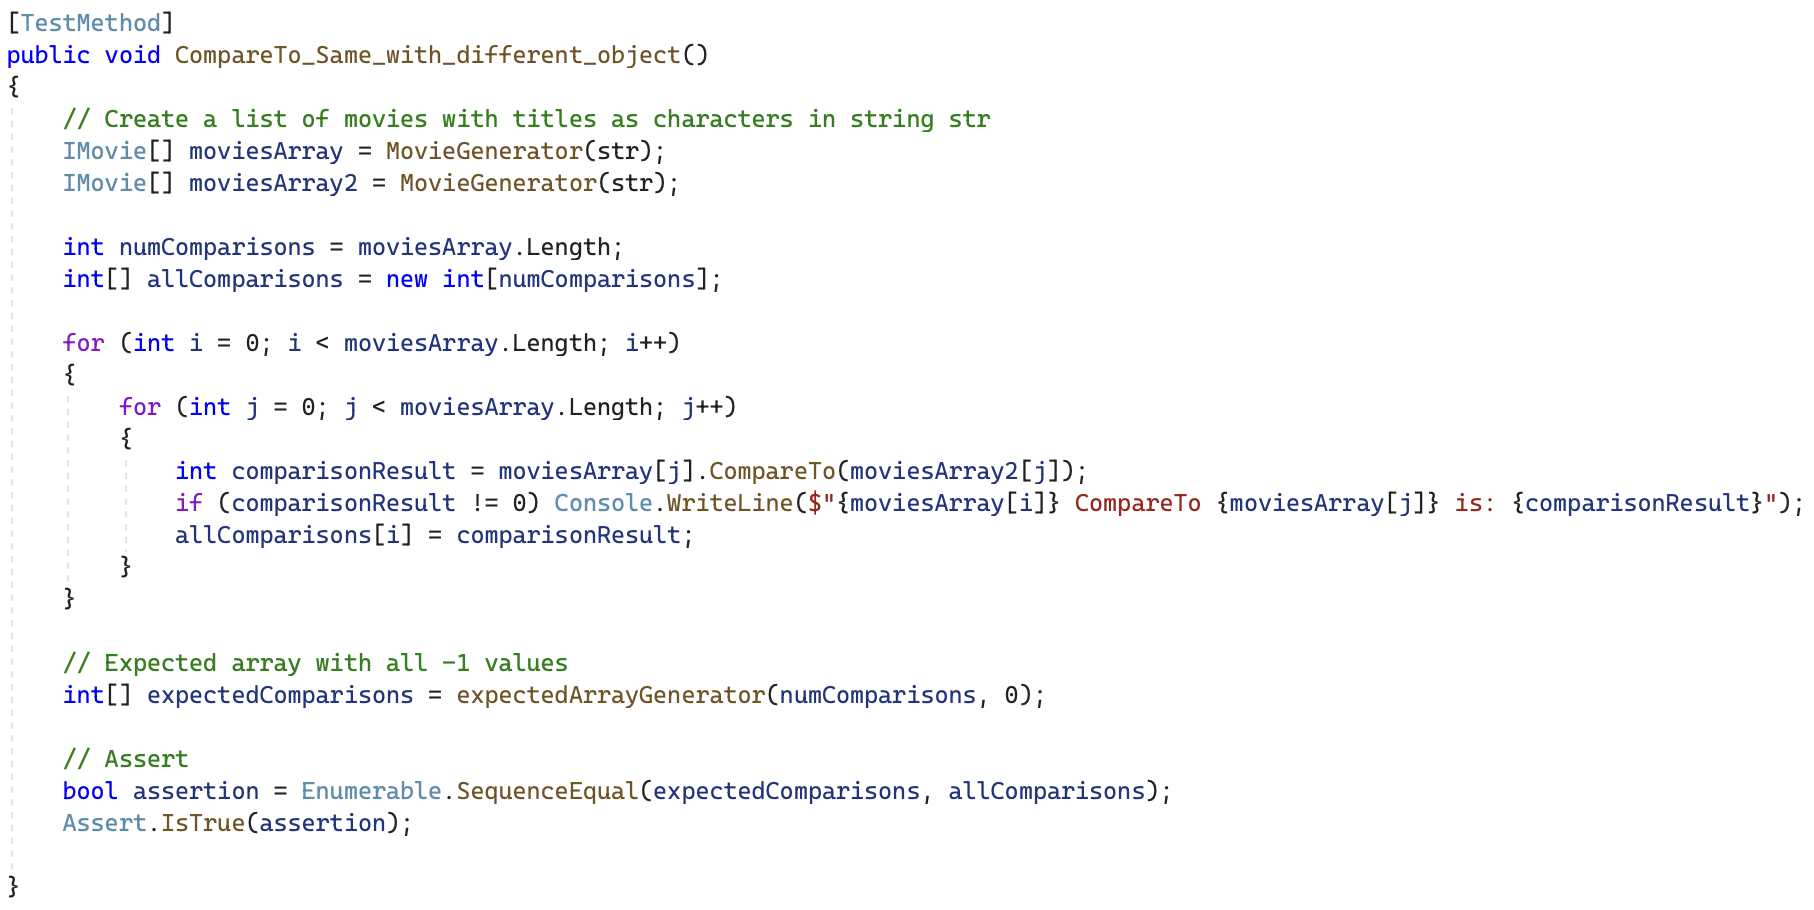
\includegraphics[height=8cm]{data/CompareTo_Same_with_different_object.png}
    \caption{Test for testing if $0$ is outputted correctly for all possible comparisons}
\end{figure}
\pagebreak

\subsubsection{ToString{()}}
\hyperlink{subsubsection.3.1.2}{Back to test plan for ToString}.
\begin{figure}[H]
    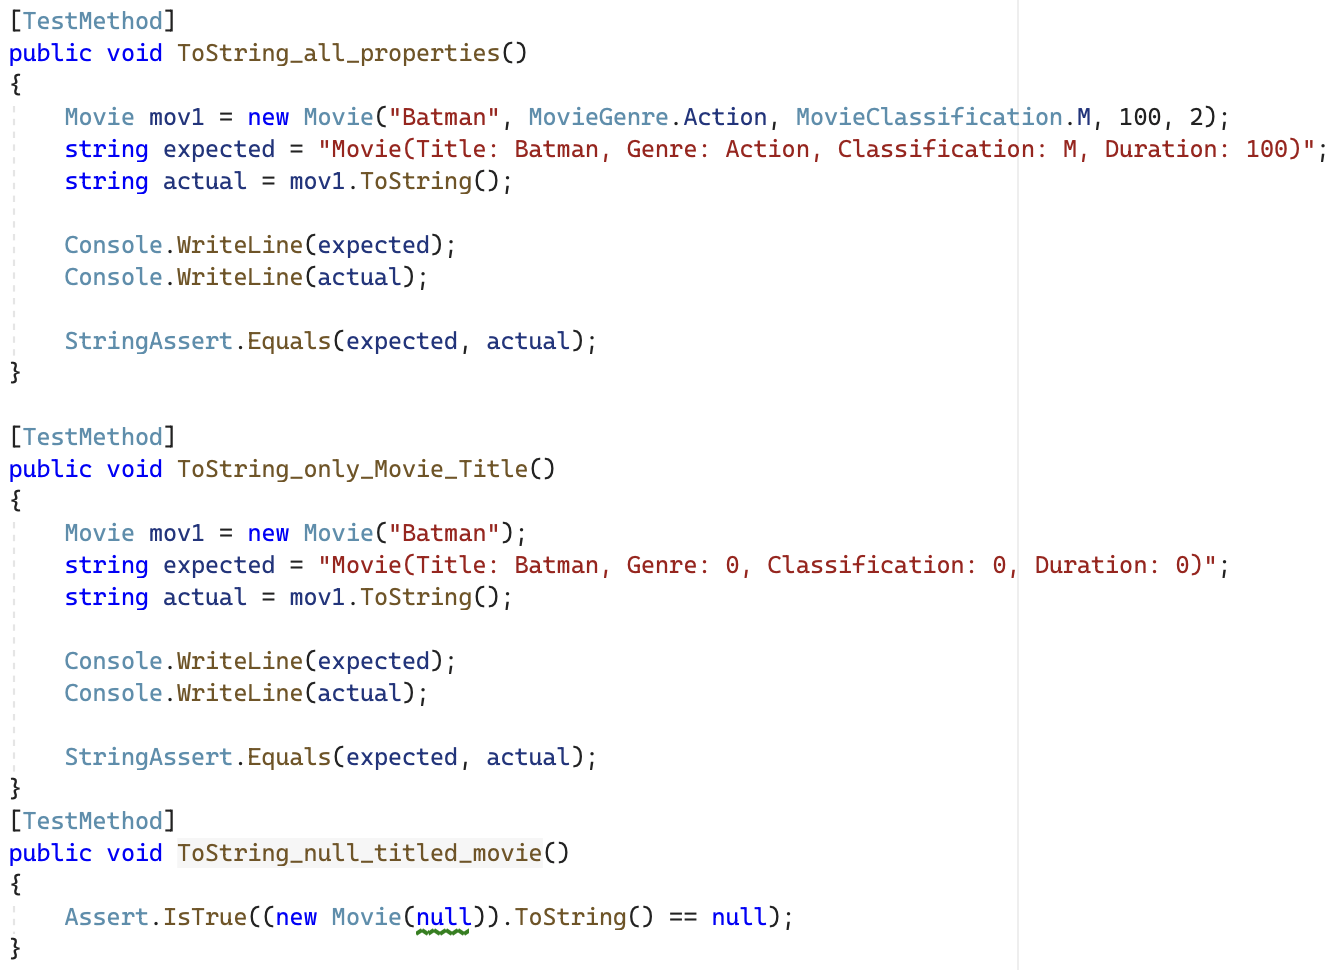
\includegraphics[height=8cm]{data/ToString-tests.png}
    \caption{Test for testing if $0$ is outputted correctly for all possible comparisons}
\end{figure}


\subsection{MovieCollection ADT}

\subsubsection{IsEmpty{()}}
\hyperlink{subsubsection.3.2.1}{Back to test plan for IsEmpty}.
\begin{figure}[H]
    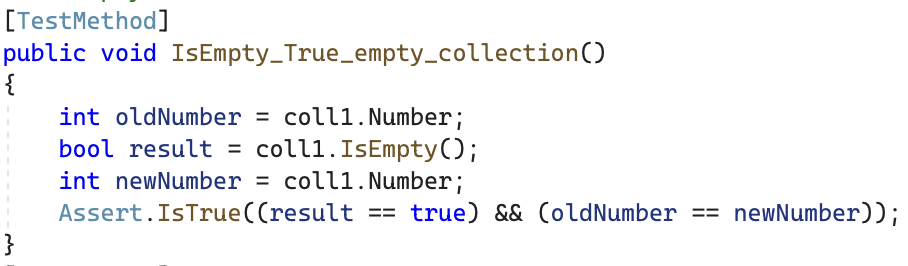
\includegraphics[height=3cm]{data/IsEmpty-True-empty.png}
    \caption{Testing when collection is empty}
\end{figure}
\begin{figure}[H]
    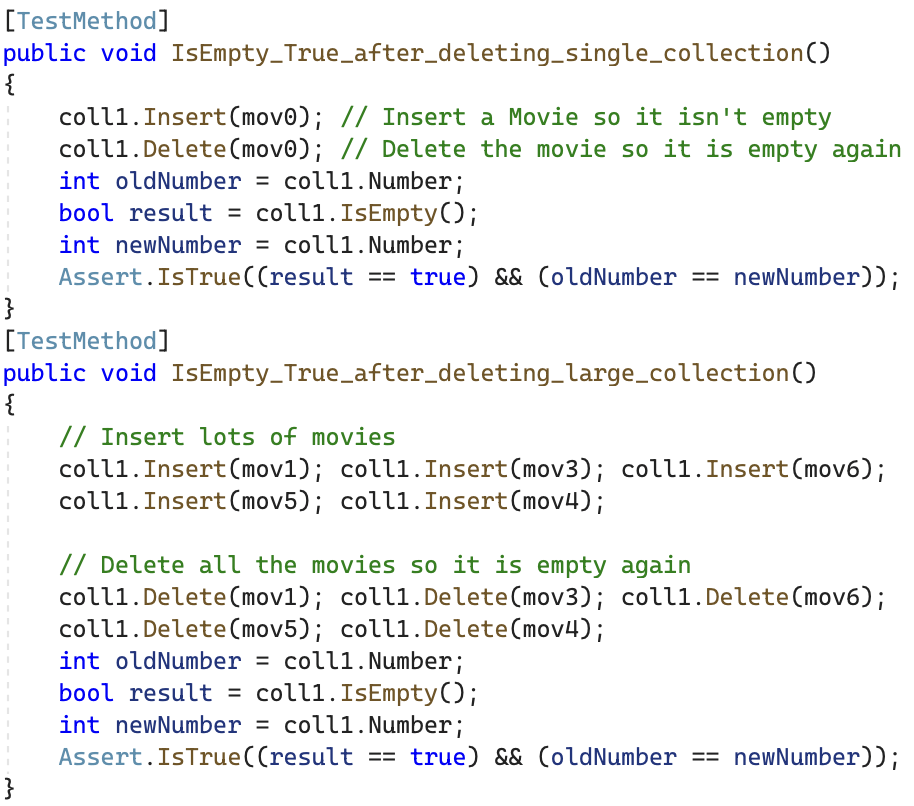
\includegraphics[height=8cm]{data/IsEmpty-True-single-large.png}
    \caption{Testing when a \textit{single} or \textit{large} collection are emptied}
\end{figure}
\begin{figure}[H]
    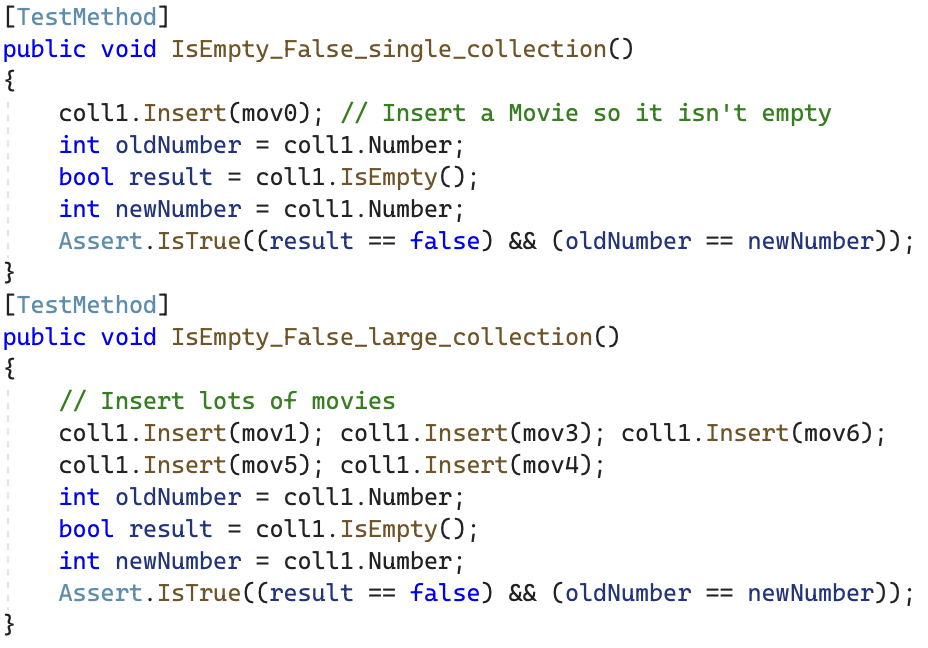
\includegraphics[height=8cm]{data/IsEmpty-False-single-large.png}
    \caption{Testing for non-empty \textit{single} or \textit{large} collections}
\end{figure}

\subsubsection{Insert{(IMovie movie)}}
\hyperlink{subsubsection.3.2.2}{Back to test plan for Insert}.
\begin{figure}[H]
    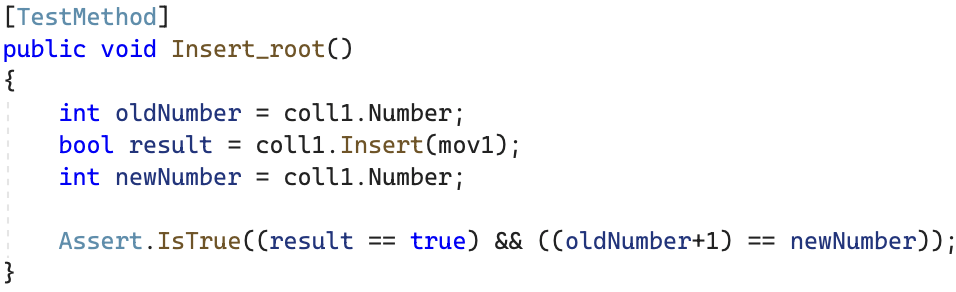
\includegraphics[height=3.5cm]{data/Insert_root.png}
    \caption{Inserting root into empty collection}
\end{figure}
\begin{figure}[H]
    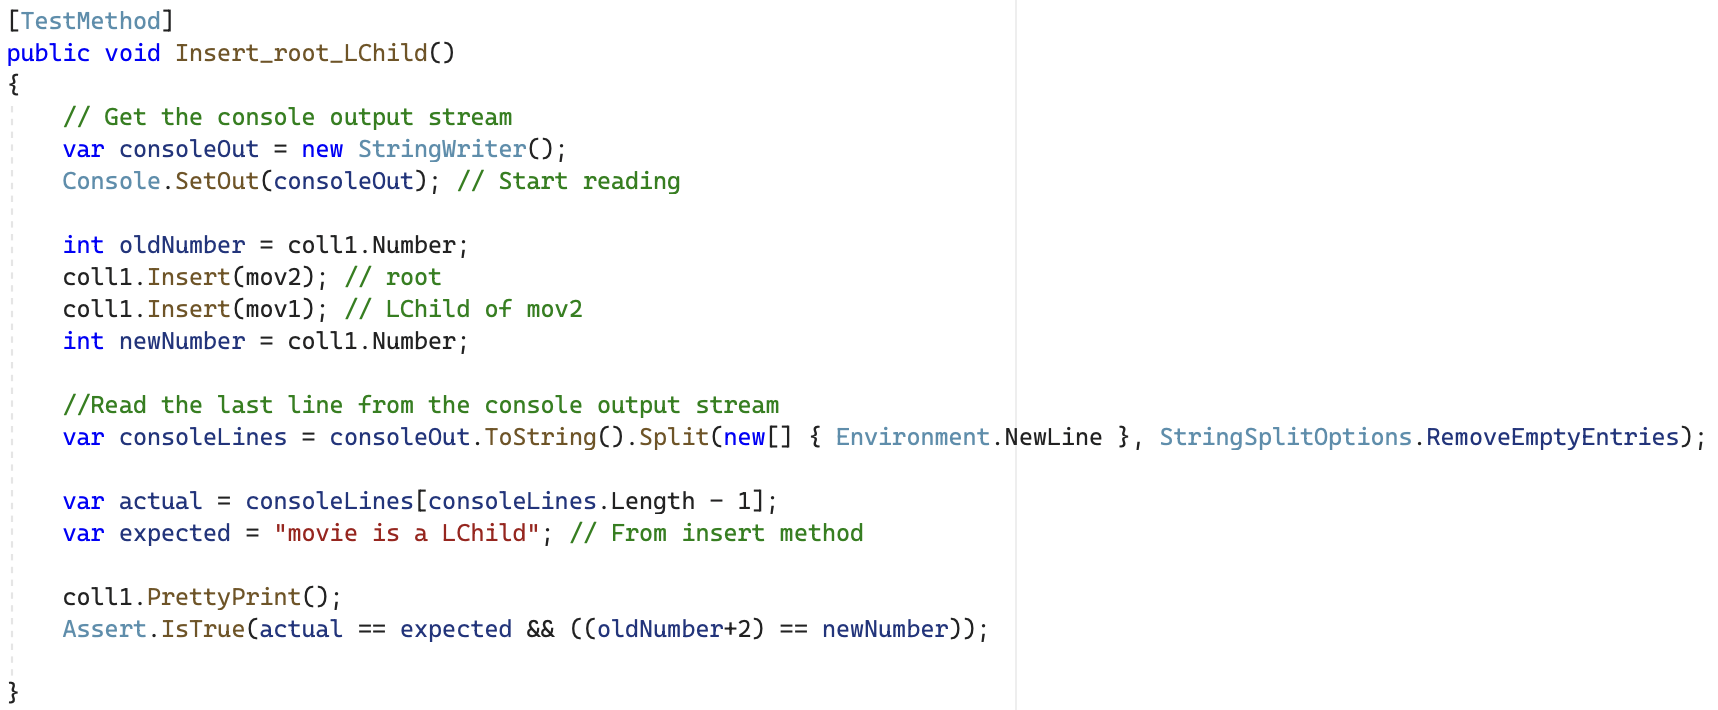
\includegraphics[height=7cm]{data/Insert_root_LChild.png}
    \caption{Inserting an LChild of a root}
\end{figure}
\begin{figure}[H]
    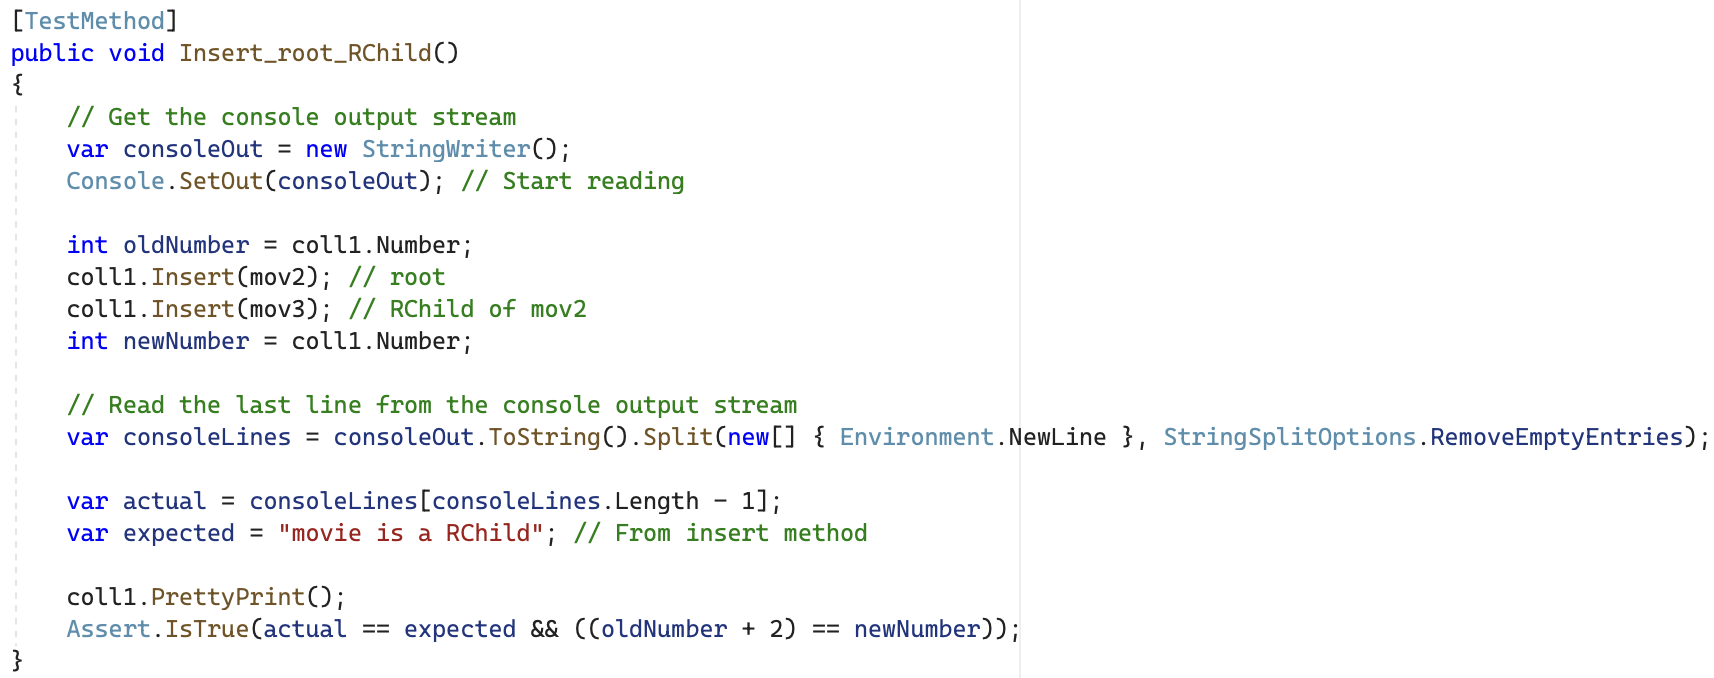
\includegraphics[height=7cm]{data/Insert_root_RChild.png}
    \caption{Inserting an RChild of a root}
\end{figure}
\begin{figure}[H]
    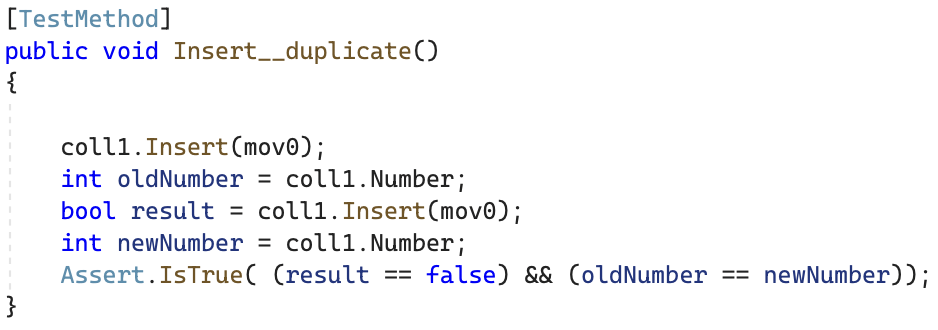
\includegraphics[height=4cm]{data/Insert__duplicate.png}
    \caption{Inserting a duplicate movie into a collection}
\end{figure}
\begin{figure}[H]
    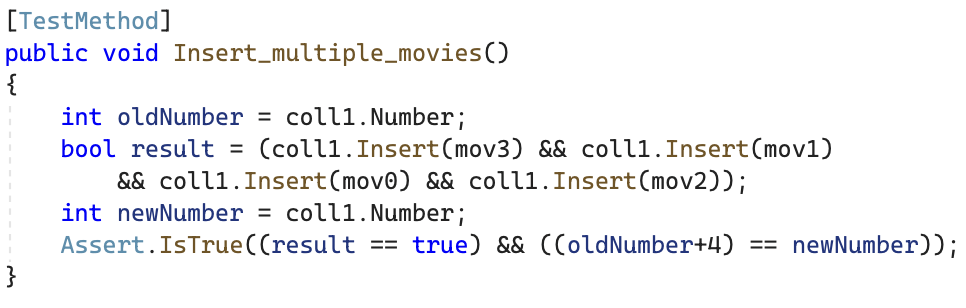
\includegraphics[height=4cm]{data/Insert_multiple_movies.png}
    \caption{Inserting multiple movies into a collection}
\end{figure}

\subsubsection{ToArray{()}}
\hyperlink{subsubsection.3.2.3}{Back to test plan for ToArray}.
\begin{figure}[H]
    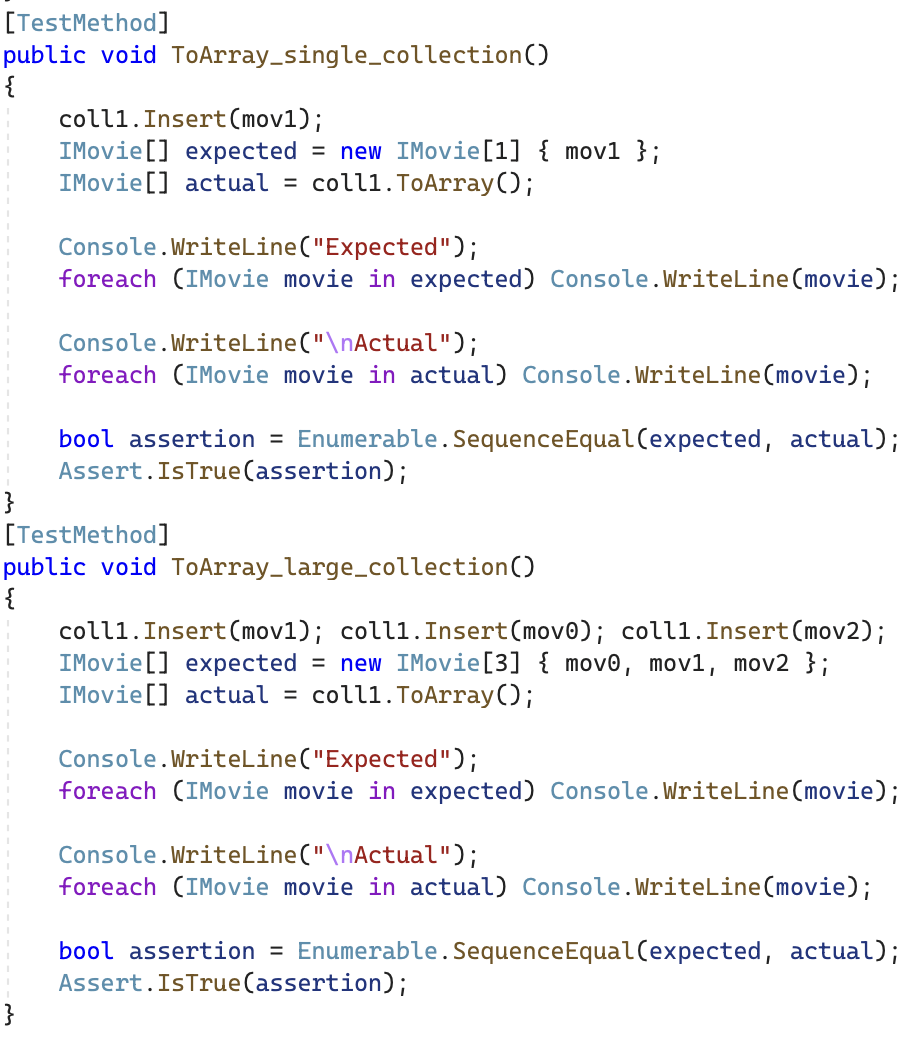
\includegraphics[height=11cm]{data/ToArray_single_large.png}
    \caption{ToArray for a single and large collection}
\end{figure}
\begin{figure}[H]
    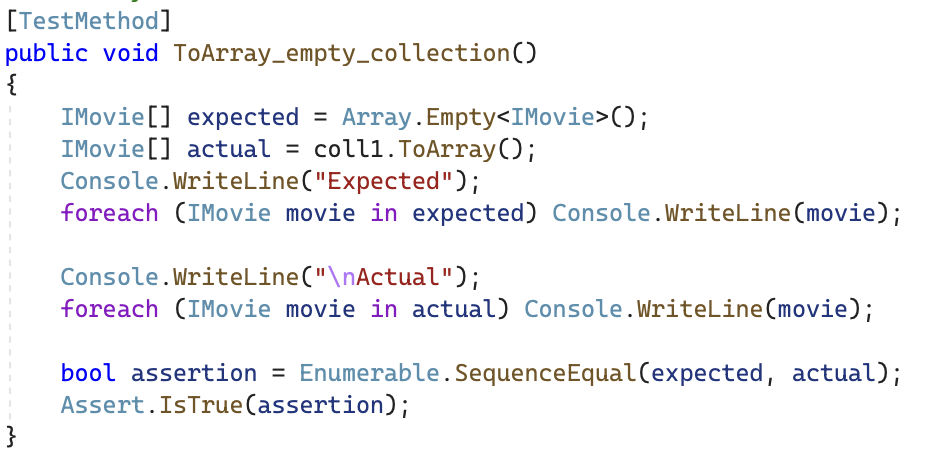
\includegraphics[height=5cm]{data/ToArray_empty_collection.png}
    \caption{ToArray for an empty collection}
\end{figure}

\subsubsection{Search{(string title)}}
\hyperlink{subsubsection.3.2.4}{Back to test plan for Search}.
\begin{figure}[H]
    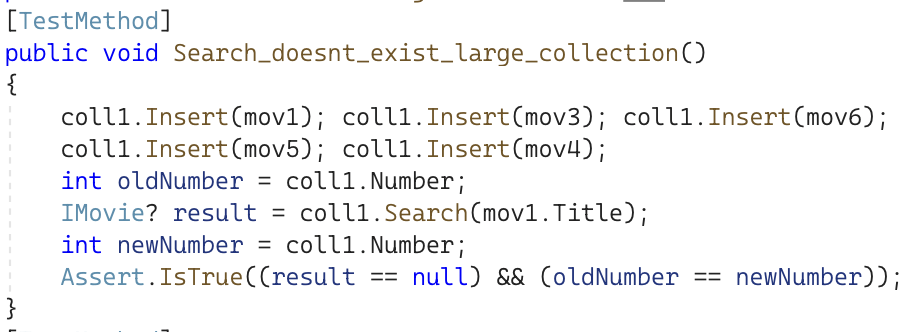
\includegraphics[height=4cm]{data/Search_doesnt_exist_large_collection.png}
    \caption{Searching for mov1 in a large collection that doesn't have it}
\end{figure}
\begin{figure}[H]
    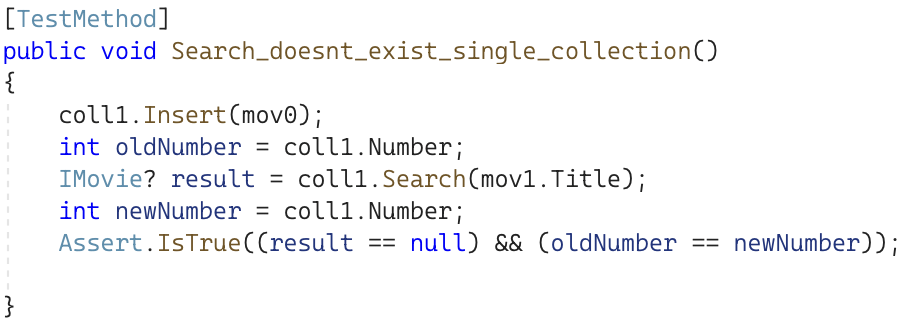
\includegraphics[height=4cm]{data/Search_doesnt_exist_single_collection.png}
    \caption{Searching for mov1 in a single collection that doesn't have it}
\end{figure}
\begin{figure}[H]
    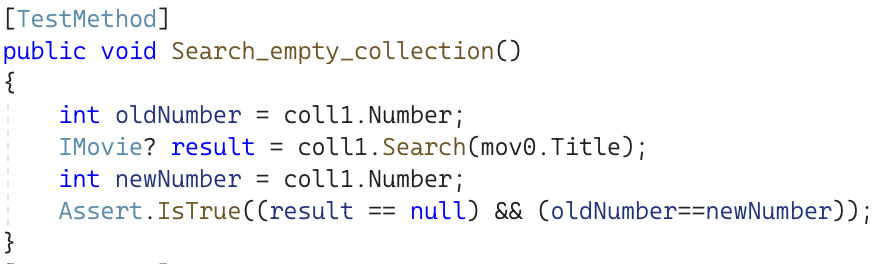
\includegraphics[height=4cm]{data/Search_empty_collection.png}
    \caption{Searching for mov0 in an empty collection}
\end{figure}
\begin{figure}[H]
    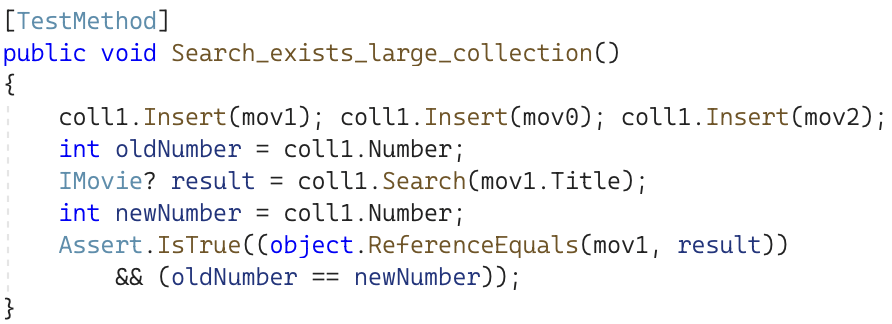
\includegraphics[height=4cm]{data/Search_exists_large_collection.png}
    \caption{Searching for mov1 in a large collection that has it}
\end{figure}
\begin{figure}[H]
    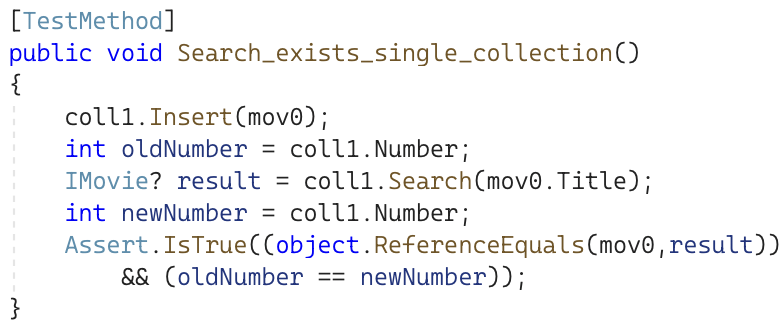
\includegraphics[height=4cm]{data/Search_exists_single_collection.png}
    \caption{Searching for mov0 in a large collection that has it}
\end{figure}
\begin{figure}[H]
    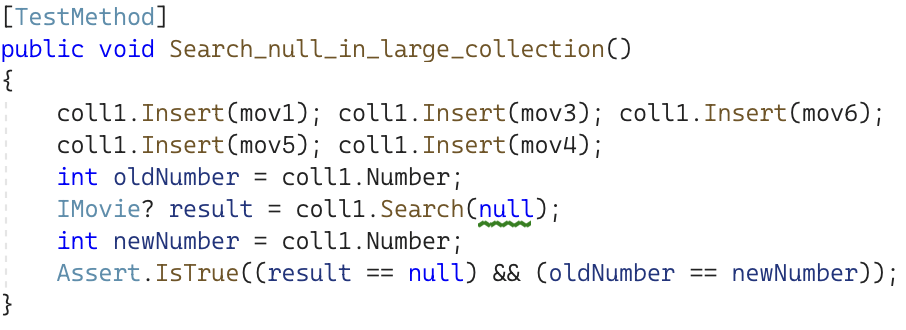
\includegraphics[height=4cm]{data/Search_null_in_large_collection.png}
    \caption{Searching for null in a large collection}
\end{figure}
\begin{figure}[H]
    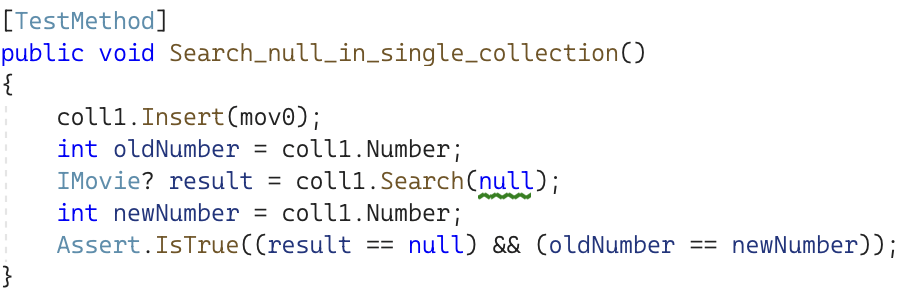
\includegraphics[height=4cm]{data/Search_null_in_single_collection.png}
    \caption{Searching for null in a single collection}
\end{figure}
\pagebreak

\subsubsection{Delete{(IMovie movie)}}
\hyperlink{subsubsection.3.2.5}{Back to test plan for Delete}.

\begin{figure}[H]
    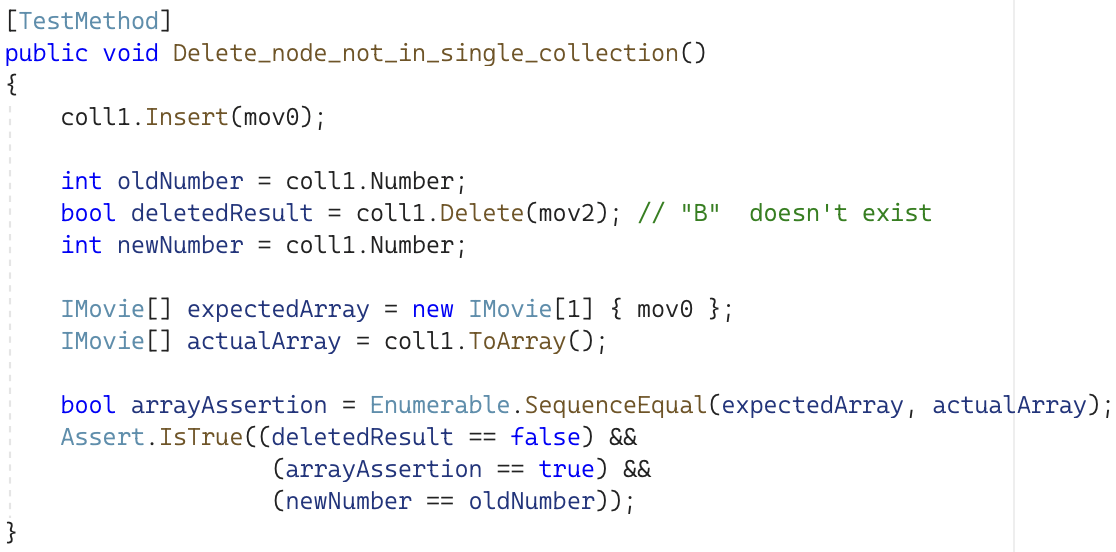
\includegraphics[height=6cm]{data/Delete_node_not_in_single_collection.png}
    \caption{Deleting a mov0 not in a \textit{single} collection. Note that the assertion captures all post-conditions}
\end{figure}
\begin{figure}[H]
    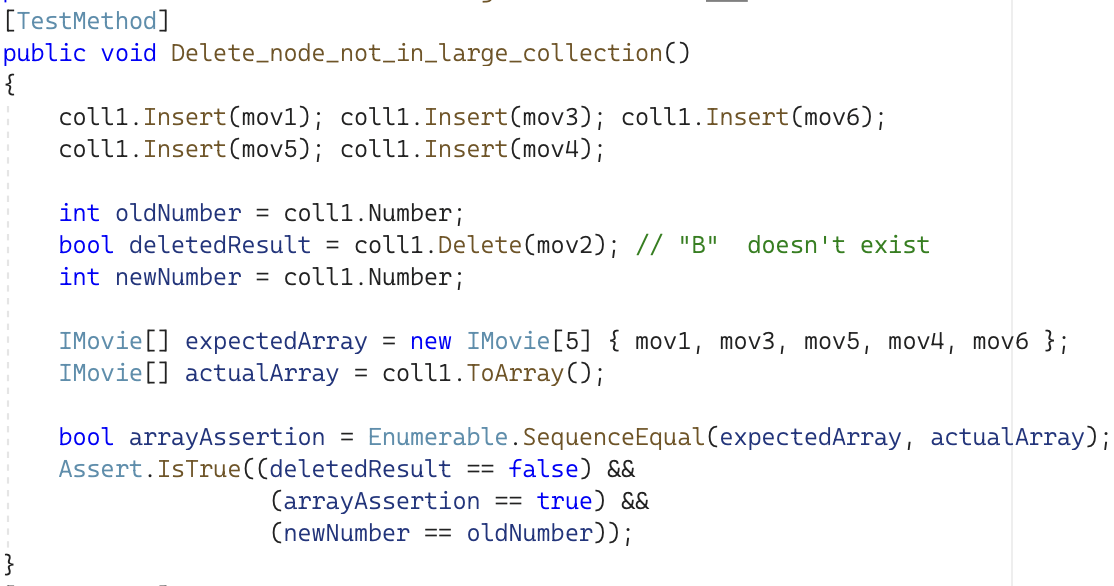
\includegraphics[height=6cm]{data/Delete_node_not_in_large_collection.png}
    \caption{Deleting a mov2 not in a \textit{large} collection.}
\end{figure}
\begin{figure}[H]
    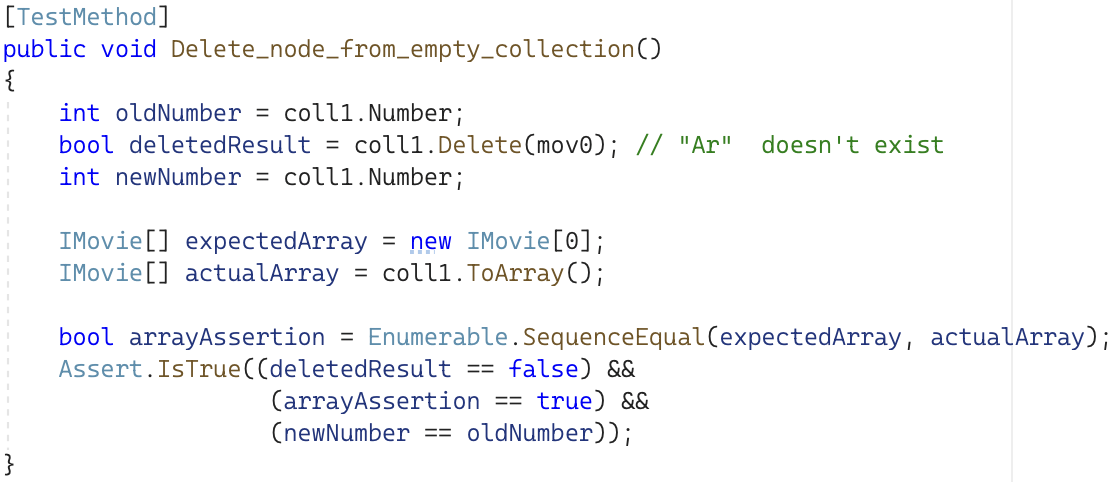
\includegraphics[height=6cm]{data/Delete_node_from_empty_collection.png}
    \caption{Deleting a mov0 not in an empty collection.}
\end{figure}
\begin{figure}[H]
    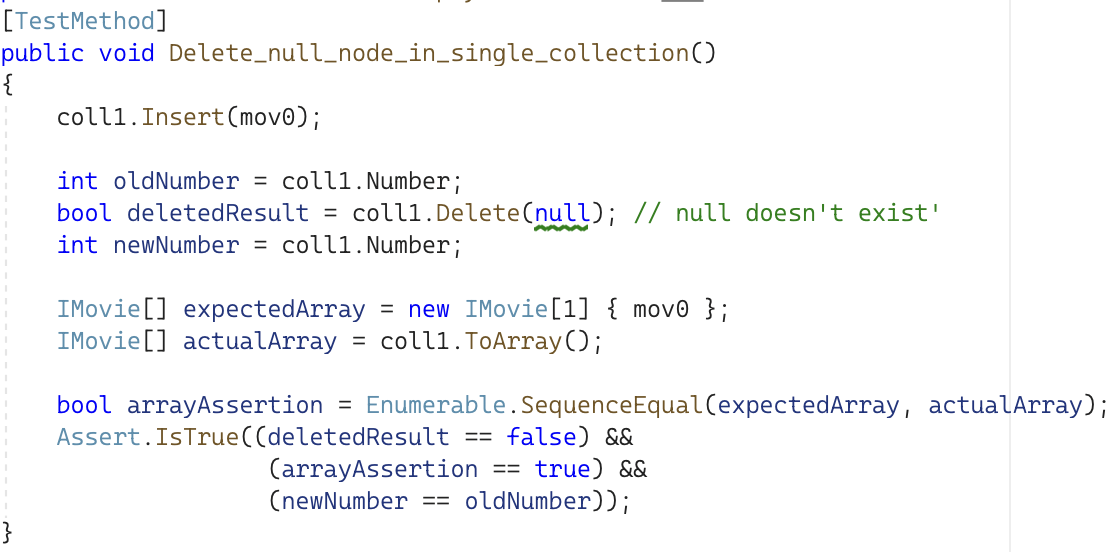
\includegraphics[height=6cm]{data/Delete_null_node_in_single_collection.png}
    \caption{Deleting a null node not in a \textit{single} collection.}
\end{figure}
\begin{figure}[H]
    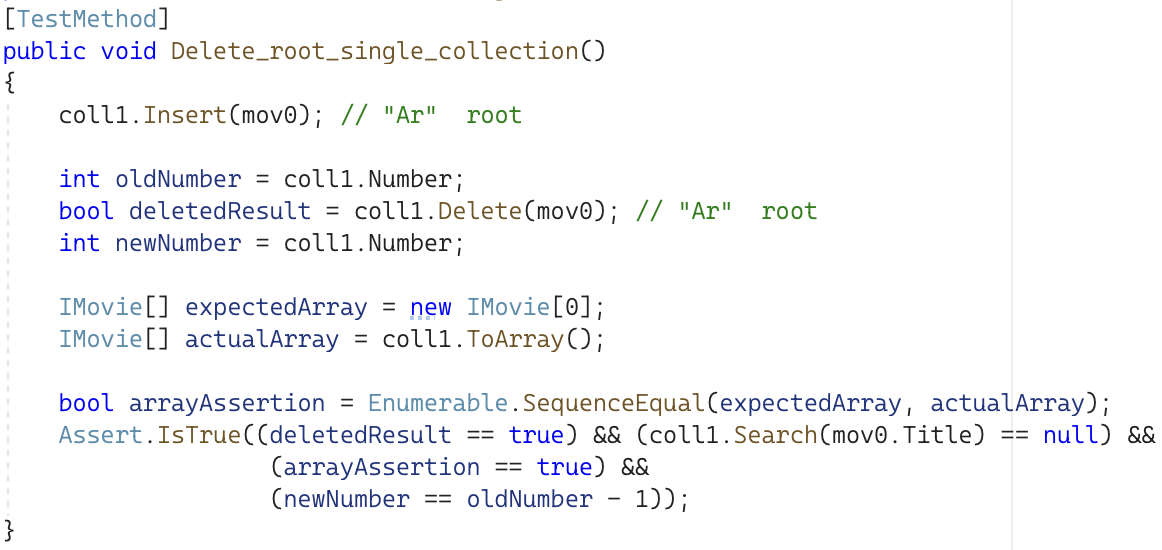
\includegraphics[height=6cm]{data/Delete_root_single_collection.png}
    \caption{Deleting the root; mov0}
\end{figure}
\begin{figure}[H]
    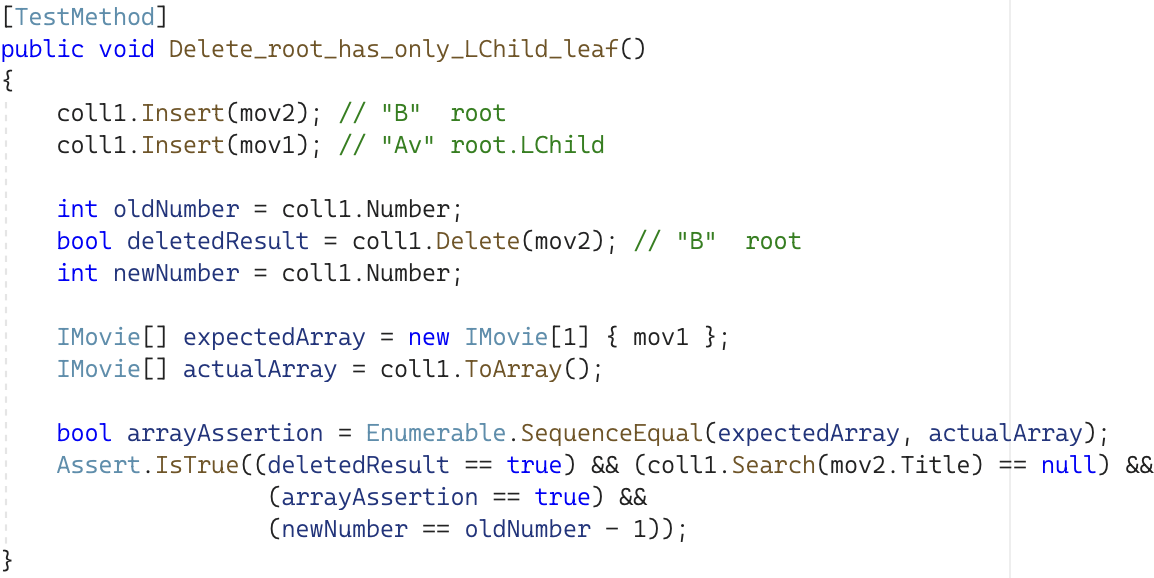
\includegraphics[height=6cm]{data/Delete_root_has_only_LChild_leaf.png}
    \caption{Deleting the root; mov2}
\end{figure}
\begin{figure}[H]
    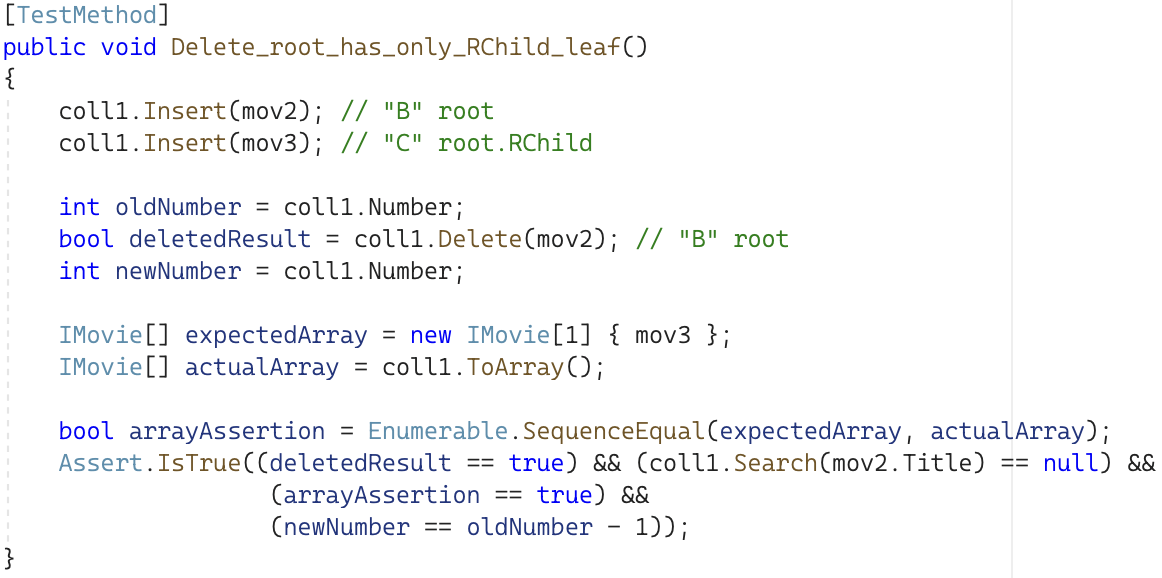
\includegraphics[height=6cm]{data/Delete_root_has_only_RChild_leaf.png}
    \caption{Deleting the root; mov2}
\end{figure}
\begin{figure}[H]
    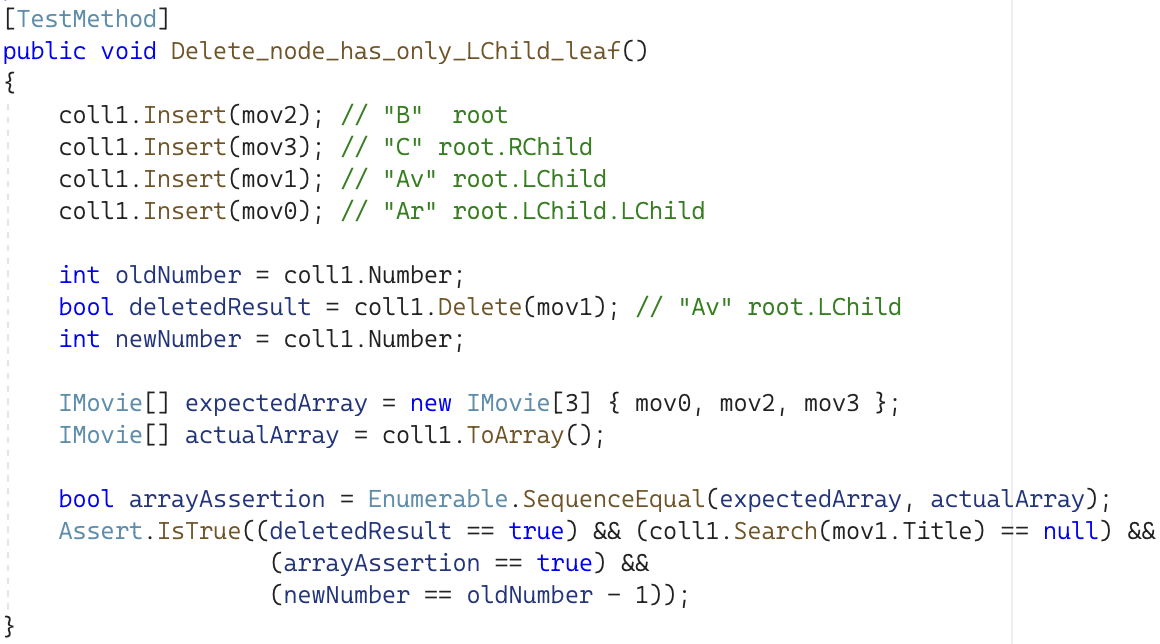
\includegraphics[height=6cm]{data/Delete_node_has_only_LChild_leaf.png}
    \caption{Deleting the node; mov1}
\end{figure}
\begin{figure}[H]
    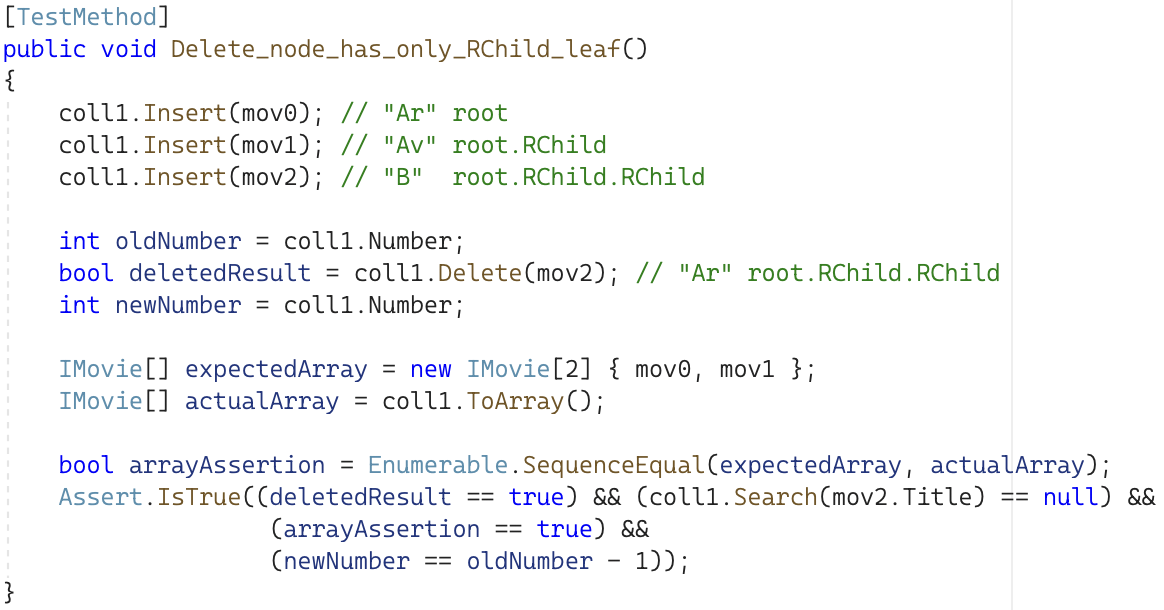
\includegraphics[height=6cm]{data/Delete_node_has_only_RChild_leaf.png}
    \caption{Deleting the node; mov2}
\end{figure}
\begin{figure}[H]
    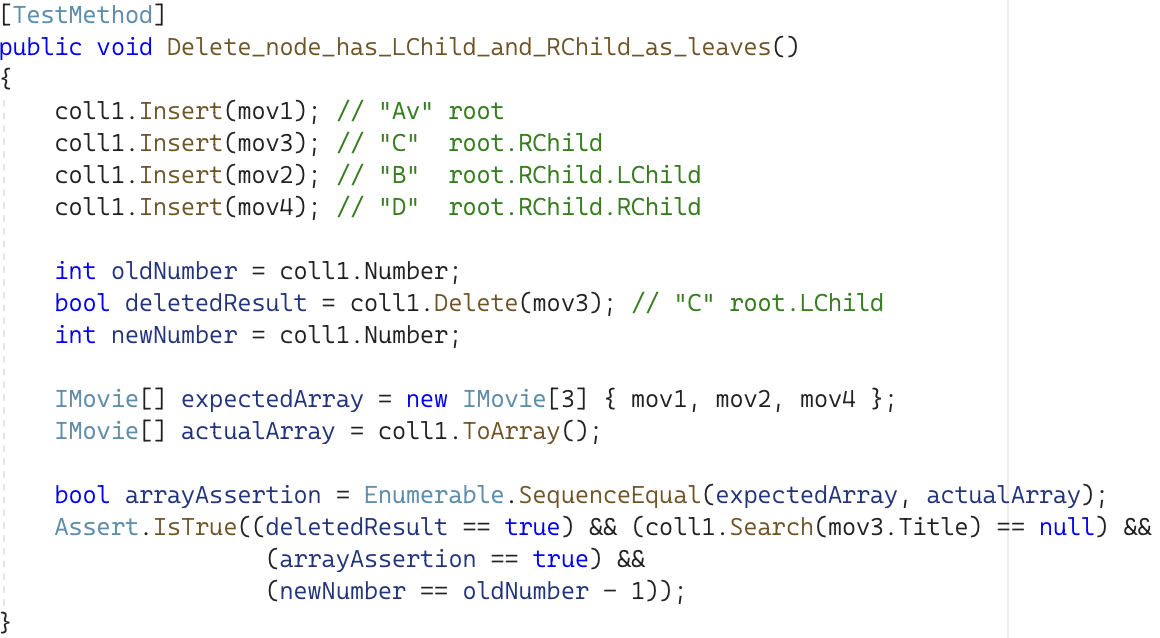
\includegraphics[height=6cm]{data/Delete_node_has_LChild_and_RChild_as_leaves.png}
    \caption{Deleting the node; mov3}
\end{figure}
\begin{figure}[H]
    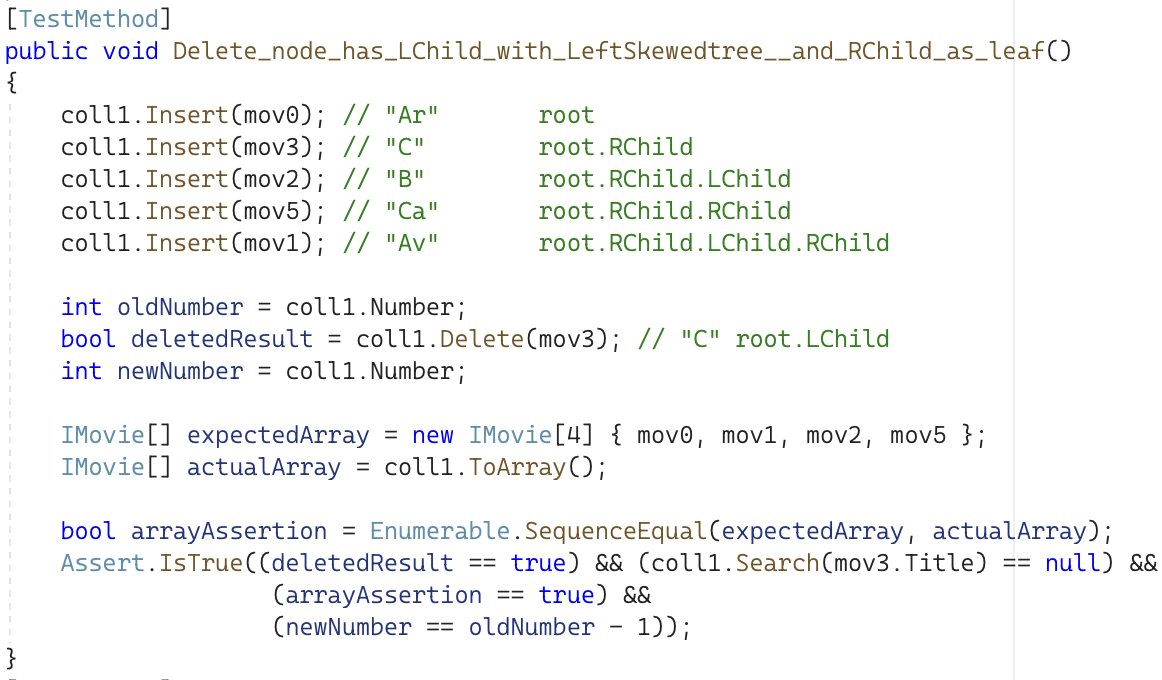
\includegraphics[height=6cm]{data/Delete_node_has_LChild_with_LeftSkewedtree__and_RChild_as_leaf.png}
    \caption{Deleting the node; mov3}
\end{figure}
\begin{figure}[H]
    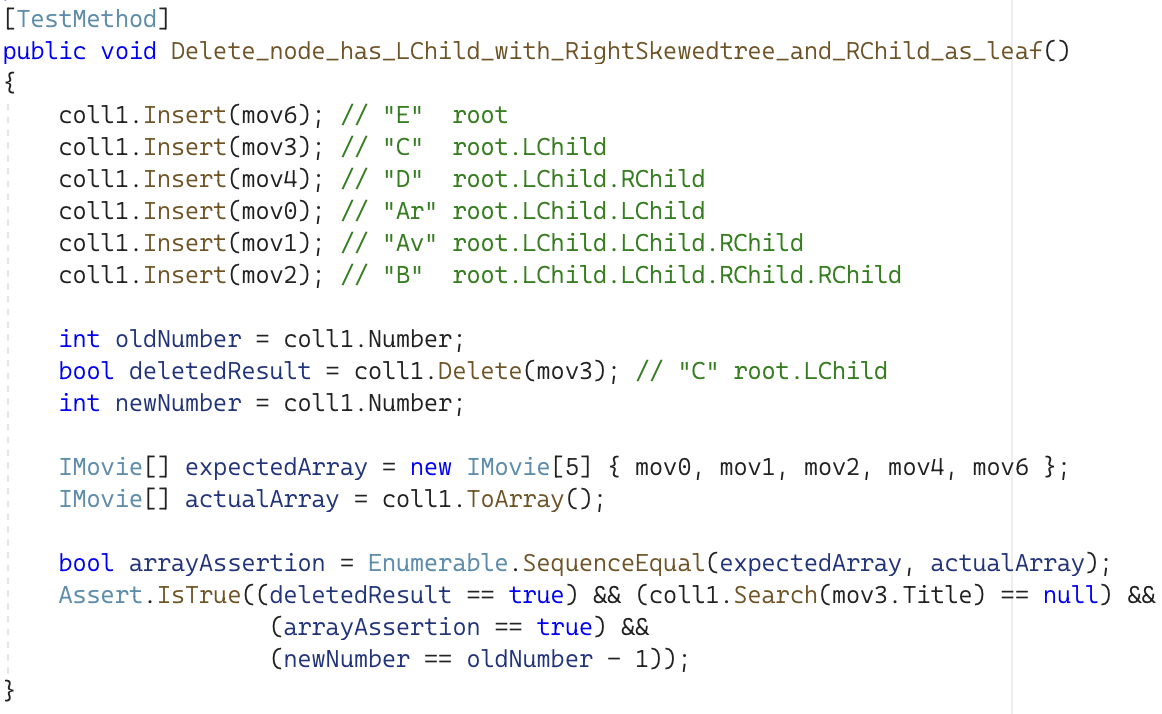
\includegraphics[height=6cm]{data/Delete_node_has_LChild_with_RightSkewedtree_and_RChild_as_leaf.png}
    \caption{Deleting the node; mov3}
\end{figure}

\pagebreak

\subsubsection{Clear{()}}
\hyperlink{subsubsection.3.2.6}{Back to test plan for Clear}.

\begin{figure}[H]
    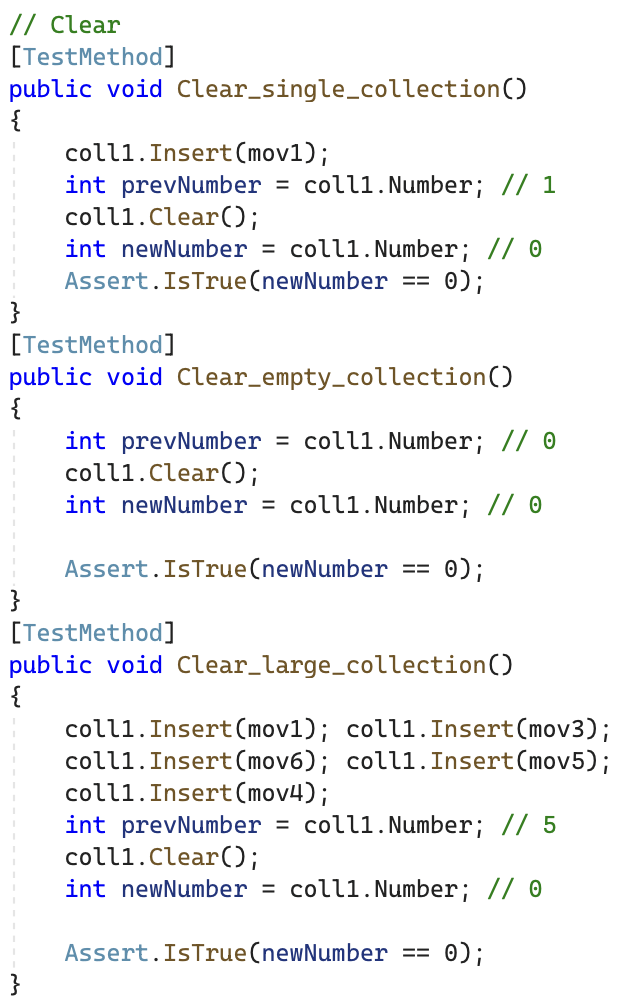
\includegraphics[height=10cm]{data/Clear-code.png}
    \caption{Clear works in all three scenarios}
\end{figure}

\subsubsection{NoDVDs{()}}
\hyperlink{subsubsection.3.2.7}{Back to test plan for NoDVDs}.

\begin{figure}[H]
    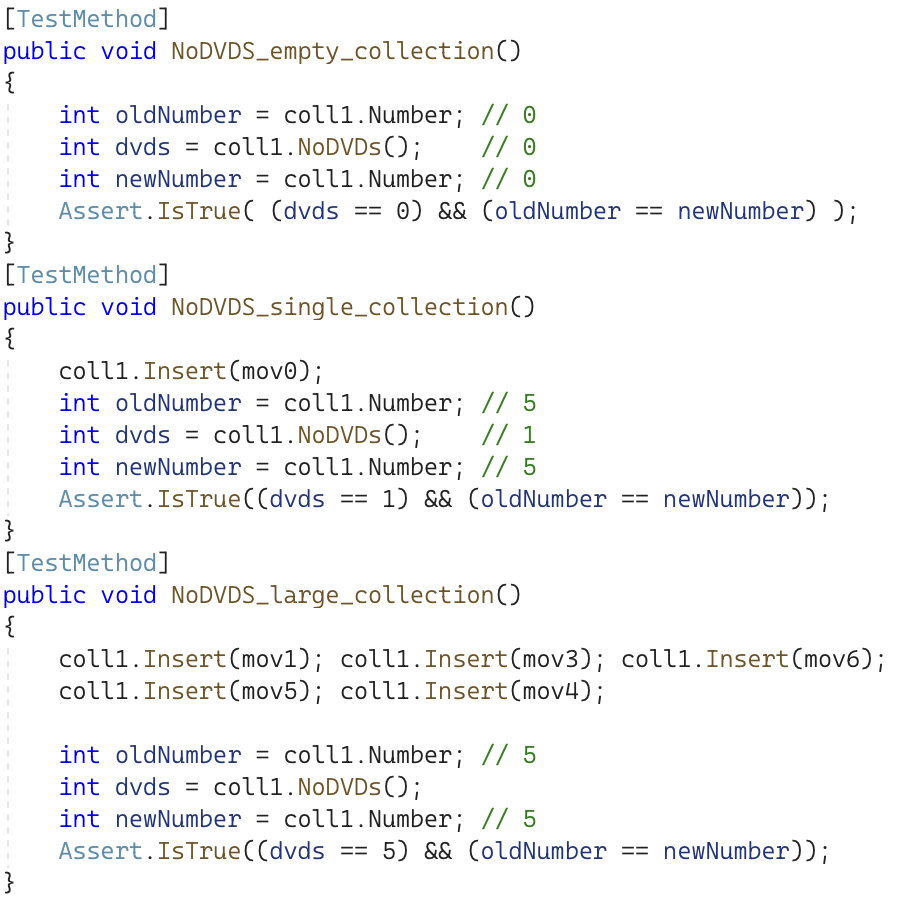
\includegraphics[height=9.5cm]{data/NoDVDs-code.png}
    \caption{NoDVDs and post-condtion is correct for all 3 tests}
\end{figure}

\end{document}